\documentclass{slides}
\usepackage{xspace}
\usepackage{nth}
\usepackage{fontawesome}
\usepackage{hyperref}
\hypersetup{
    colorlinks = true,
    urlcolor = blue
}

\title[Bayesian Inference]{Inference in a Poisson model}
\author[Andrews]{Mark Andrews \\ $\phantom{foo}$ \\ Psychology, Nottingham Trent University \\ $\phantom{foo}$ \\ \faEnvelopeO \  \texttt{mark.andrews@ntu.ac.uk} \\ $\phantom{foo}$ \\ \faTwitter \href{https://twitter.com/xmjandrews}{@xmjandrews}, \faTwitter \href{https://twitter.com/priorexposure}{@priorexposure}\\ $\phantom{foo}$ \\ \faGithub \ \url{https://github.com/lawsofthought/psbayes}}

\date{December, 2018}

\begin{document}
{
	\begin{frame}
		\titlepage
	\end{frame}
}


	\begin{frame}
		\frametitle{Inference in Poisson models}
		\begin{itemize}
			\item The Poisson distribution can be used to model the rare occurrences in fixed intervals.
			\item If $x$ is a Poisson random variable with rate $\lambda$, then 
				\[\Prob{x = k \given \lambda} = \frac{\lambda^k e^{-\lambda}}{k!}.\]
		\end{itemize}
		% Created by tikzDevice version 0.12 on 2018-12-03 08:01:45
% !TEX encoding = UTF-8 Unicode
\begin{tikzpicture}[x=1pt,y=1pt]
\definecolor{fillColor}{RGB}{255,255,255}
\path[use as bounding box,fill=fillColor,fill opacity=0.00] (0,0) rectangle (274.17,164.50);
\begin{scope}
\path[clip] ( 60.00, 48.00) rectangle (274.17,152.50);
\definecolor{drawColor}{RGB}{210,105,30}

\path[draw=drawColor,line width= 0.4pt,line join=round,line cap=round] ( 67.93, 51.87) -- ( 67.93, 55.49);

\path[draw=drawColor,line width= 0.4pt,line join=round,line cap=round] ( 81.15, 51.87) -- ( 81.15, 69.98);

\path[draw=drawColor,line width= 0.4pt,line join=round,line cap=round] ( 94.37, 51.87) -- ( 94.37, 97.15);

\path[draw=drawColor,line width= 0.4pt,line join=round,line cap=round] (107.59, 51.87) -- (107.59,127.33);

\path[draw=drawColor,line width= 0.4pt,line join=round,line cap=round] (120.81, 51.87) -- (120.81,146.20);

\path[draw=drawColor,line width= 0.4pt,line join=round,line cap=round] (134.03, 51.87) -- (134.03,146.20);

\path[draw=drawColor,line width= 0.4pt,line join=round,line cap=round] (147.25, 51.87) -- (147.25,130.47);

\path[draw=drawColor,line width= 0.4pt,line join=round,line cap=round] (160.48, 51.87) -- (160.48,108.02);

\path[draw=drawColor,line width= 0.4pt,line join=round,line cap=round] (173.70, 51.87) -- (173.70, 86.96);

\path[draw=drawColor,line width= 0.4pt,line join=round,line cap=round] (186.92, 51.87) -- (186.92, 71.37);

\path[draw=drawColor,line width= 0.4pt,line join=round,line cap=round] (200.14, 51.87) -- (200.14, 61.62);

\path[draw=drawColor,line width= 0.4pt,line join=round,line cap=round] (213.36, 51.87) -- (213.36, 56.30);

\path[draw=drawColor,line width= 0.4pt,line join=round,line cap=round] (226.58, 51.87) -- (226.58, 53.72);

\path[draw=drawColor,line width= 0.4pt,line join=round,line cap=round] (239.80, 51.87) -- (239.80, 52.58);

\path[draw=drawColor,line width= 0.4pt,line join=round,line cap=round] (253.02, 51.87) -- (253.02, 52.12);

\path[draw=drawColor,line width= 0.4pt,line join=round,line cap=round] (266.24, 51.87) -- (266.24, 51.95);
\end{scope}
\begin{scope}
\path[clip] (  0.00,  0.00) rectangle (274.17,164.50);
\definecolor{drawColor}{RGB}{0,0,0}

\path[draw=drawColor,line width= 0.4pt,line join=round,line cap=round] ( 67.93, 48.00) -- (266.24, 48.00);

\path[draw=drawColor,line width= 0.4pt,line join=round,line cap=round] ( 67.93, 48.00) -- ( 67.93, 42.00);

\path[draw=drawColor,line width= 0.4pt,line join=round,line cap=round] ( 81.15, 48.00) -- ( 81.15, 42.00);

\path[draw=drawColor,line width= 0.4pt,line join=round,line cap=round] ( 94.37, 48.00) -- ( 94.37, 42.00);

\path[draw=drawColor,line width= 0.4pt,line join=round,line cap=round] (107.59, 48.00) -- (107.59, 42.00);

\path[draw=drawColor,line width= 0.4pt,line join=round,line cap=round] (120.81, 48.00) -- (120.81, 42.00);

\path[draw=drawColor,line width= 0.4pt,line join=round,line cap=round] (134.03, 48.00) -- (134.03, 42.00);

\path[draw=drawColor,line width= 0.4pt,line join=round,line cap=round] (147.25, 48.00) -- (147.25, 42.00);

\path[draw=drawColor,line width= 0.4pt,line join=round,line cap=round] (160.48, 48.00) -- (160.48, 42.00);

\path[draw=drawColor,line width= 0.4pt,line join=round,line cap=round] (173.70, 48.00) -- (173.70, 42.00);

\path[draw=drawColor,line width= 0.4pt,line join=round,line cap=round] (186.92, 48.00) -- (186.92, 42.00);

\path[draw=drawColor,line width= 0.4pt,line join=round,line cap=round] (200.14, 48.00) -- (200.14, 42.00);

\path[draw=drawColor,line width= 0.4pt,line join=round,line cap=round] (213.36, 48.00) -- (213.36, 42.00);

\path[draw=drawColor,line width= 0.4pt,line join=round,line cap=round] (226.58, 48.00) -- (226.58, 42.00);

\path[draw=drawColor,line width= 0.4pt,line join=round,line cap=round] (239.80, 48.00) -- (239.80, 42.00);

\path[draw=drawColor,line width= 0.4pt,line join=round,line cap=round] (253.02, 48.00) -- (253.02, 42.00);

\path[draw=drawColor,line width= 0.4pt,line join=round,line cap=round] (266.24, 48.00) -- (266.24, 42.00);

\node[text=drawColor,anchor=base,inner sep=0pt, outer sep=0pt, scale=  1.00] at ( 67.93, 26.40) {0};

\node[text=drawColor,anchor=base,inner sep=0pt, outer sep=0pt, scale=  1.00] at ( 94.37, 26.40) {2};

\node[text=drawColor,anchor=base,inner sep=0pt, outer sep=0pt, scale=  1.00] at (120.81, 26.40) {4};

\node[text=drawColor,anchor=base,inner sep=0pt, outer sep=0pt, scale=  1.00] at (147.25, 26.40) {6};

\node[text=drawColor,anchor=base,inner sep=0pt, outer sep=0pt, scale=  1.00] at (173.70, 26.40) {8};

\node[text=drawColor,anchor=base,inner sep=0pt, outer sep=0pt, scale=  1.00] at (200.14, 26.40) {10};

\node[text=drawColor,anchor=base,inner sep=0pt, outer sep=0pt, scale=  1.00] at (226.58, 26.40) {12};

\node[text=drawColor,anchor=base,inner sep=0pt, outer sep=0pt, scale=  1.00] at (253.02, 26.40) {14};

\node[text=drawColor,anchor=base,inner sep=0pt, outer sep=0pt, scale=  1.00] at (167.09,  2.40) {$\lambda$};

\path[draw=drawColor,line width= 0.4pt,line join=round,line cap=round] ( 60.00, 51.87) -- ( 60.00,132.51);

\path[draw=drawColor,line width= 0.4pt,line join=round,line cap=round] ( 60.00, 51.87) -- ( 54.00, 51.87);

\path[draw=drawColor,line width= 0.4pt,line join=round,line cap=round] ( 60.00, 78.75) -- ( 54.00, 78.75);

\path[draw=drawColor,line width= 0.4pt,line join=round,line cap=round] ( 60.00,105.63) -- ( 54.00,105.63);

\path[draw=drawColor,line width= 0.4pt,line join=round,line cap=round] ( 60.00,132.51) -- ( 54.00,132.51);

\node[text=drawColor,anchor=base east,inner sep=0pt, outer sep=0pt, scale=  1.00] at ( 48.00, 48.43) {0};

\node[text=drawColor,anchor=base east,inner sep=0pt, outer sep=0pt, scale=  1.00] at ( 48.00, 75.31) {0.05};

\node[text=drawColor,anchor=base east,inner sep=0pt, outer sep=0pt, scale=  1.00] at ( 48.00,102.18) {0.1};

\node[text=drawColor,anchor=base east,inner sep=0pt, outer sep=0pt, scale=  1.00] at ( 48.00,129.06) {0.15};

\node[text=drawColor,rotate= 90.00,anchor=base,inner sep=0pt, outer sep=0pt, scale=  1.00] at (  9.60,100.25) {$\textrm{P}(x=k\vert \lambda)$};
\end{scope}
\end{tikzpicture}

	\end{frame}
	
	\begin{frame}
		\frametitle{Inference in Poisson models}
		\begin{itemize}
			\item Let's say that the number of emails I get per hour, in $n=10$ hours, is 
				\[D = 6, 8, 12,  7, 11, 14, 10, 12, 11, 16.\]
			\item We can assume that these frequencies are generated according to a Poisson process with rate $\lambda$ per hour.
			\item Given this assumption and this observed data, what is the probable value of $\lambda$?
			\item In other words, what is 
				\[
					\Prob{\lambda \given D}?
				\]
		\end{itemize}
	\end{frame}

	\begin{frame}
		\frametitle{Likelihood of a Poisson model}
		\begin{itemize}
			\item Given a known value for $\lambda$, the probability of $x_1, x_2 \cdots x_n$ is 
				\begin{align*}
					\Prob{x_1, x_2 \cdots x_n \given \lambda} &= \prod_{i=1}^n \Prob{x_i \given \lambda},\\
					&= \prod_{i=1}^n \frac{\lambda^{x_i}e^{-\lambda}}{x_i!},\\
					&\propto e^{-n\lambda}\prod_{i=1}^n \lambda^{x_i} = e^{-n\lambda} \lambda^{\sum_{i=1}^{n}x_i}.\\
					\intertext{When $D = x_1, x_2 \cdots x_n = 6, 8 \cdots 16$, the likelihood of $\lambda$ is}
					\Prob{D \given \lambda} &= e^{-n\lambda} \lambda^{S},
				\end{align*}
				where $S = \sum_{i=1}^{n} x_i = 107$.
		\end{itemize}
	\end{frame}

	\begin{frame}
		\frametitle{Likelihood of a Poisson model}
		% Created by tikzDevice version 0.12 on 2018-12-03 08:01:38
% !TEX encoding = UTF-8 Unicode
\begin{tikzpicture}[x=1pt,y=1pt]
\definecolor{fillColor}{RGB}{255,255,255}
\path[use as bounding box,fill=fillColor,fill opacity=0.00] (0,0) rectangle (274.17,178.21);
\begin{scope}
\path[clip] ( 30.00, 36.00) rectangle (274.17,178.21);
\definecolor{drawColor}{RGB}{139,76,57}

\path[draw=drawColor,line width= 0.4pt,line join=round,line cap=round] ( 39.04, 41.27) --
	( 39.27, 41.27) --
	( 39.50, 41.27) --
	( 39.72, 41.27) --
	( 39.95, 41.27) --
	( 40.17, 41.27) --
	( 40.40, 41.27) --
	( 40.63, 41.27) --
	( 40.85, 41.27) --
	( 41.08, 41.27) --
	( 41.30, 41.27) --
	( 41.53, 41.27) --
	( 41.76, 41.27) --
	( 41.98, 41.27) --
	( 42.21, 41.27) --
	( 42.43, 41.27) --
	( 42.66, 41.27) --
	( 42.89, 41.27) --
	( 43.11, 41.27) --
	( 43.34, 41.27) --
	( 43.57, 41.27) --
	( 43.79, 41.27) --
	( 44.02, 41.27) --
	( 44.24, 41.27) --
	( 44.47, 41.27) --
	( 44.70, 41.27) --
	( 44.92, 41.27) --
	( 45.15, 41.27) --
	( 45.37, 41.27) --
	( 45.60, 41.27) --
	( 45.83, 41.27) --
	( 46.05, 41.27) --
	( 46.28, 41.27) --
	( 46.50, 41.27) --
	( 46.73, 41.27) --
	( 46.96, 41.27) --
	( 47.18, 41.27) --
	( 47.41, 41.27) --
	( 47.63, 41.27) --
	( 47.86, 41.27) --
	( 48.09, 41.27) --
	( 48.31, 41.27) --
	( 48.54, 41.27) --
	( 48.76, 41.27) --
	( 48.99, 41.27) --
	( 49.22, 41.27) --
	( 49.44, 41.27) --
	( 49.67, 41.27) --
	( 49.90, 41.27) --
	( 50.12, 41.27) --
	( 50.35, 41.27) --
	( 50.57, 41.27) --
	( 50.80, 41.27) --
	( 51.03, 41.27) --
	( 51.25, 41.27) --
	( 51.48, 41.27) --
	( 51.70, 41.27) --
	( 51.93, 41.27) --
	( 52.16, 41.27) --
	( 52.38, 41.27) --
	( 52.61, 41.27) --
	( 52.83, 41.27) --
	( 53.06, 41.27) --
	( 53.29, 41.27) --
	( 53.51, 41.27) --
	( 53.74, 41.27) --
	( 53.96, 41.27) --
	( 54.19, 41.27) --
	( 54.42, 41.27) --
	( 54.64, 41.27) --
	( 54.87, 41.27) --
	( 55.10, 41.27) --
	( 55.32, 41.27) --
	( 55.55, 41.27) --
	( 55.77, 41.27) --
	( 56.00, 41.27) --
	( 56.23, 41.27) --
	( 56.45, 41.27) --
	( 56.68, 41.27) --
	( 56.90, 41.27) --
	( 57.13, 41.27) --
	( 57.36, 41.27) --
	( 57.58, 41.27) --
	( 57.81, 41.27) --
	( 58.03, 41.27) --
	( 58.26, 41.27) --
	( 58.49, 41.27) --
	( 58.71, 41.27) --
	( 58.94, 41.27) --
	( 59.16, 41.27) --
	( 59.39, 41.27) --
	( 59.62, 41.27) --
	( 59.84, 41.27) --
	( 60.07, 41.27) --
	( 60.30, 41.27) --
	( 60.52, 41.27) --
	( 60.75, 41.27) --
	( 60.97, 41.27) --
	( 61.20, 41.27) --
	( 61.43, 41.27) --
	( 61.65, 41.27) --
	( 61.88, 41.27) --
	( 62.10, 41.27) --
	( 62.33, 41.27) --
	( 62.56, 41.27) --
	( 62.78, 41.27) --
	( 63.01, 41.27) --
	( 63.23, 41.27) --
	( 63.46, 41.27) --
	( 63.69, 41.27) --
	( 63.91, 41.27) --
	( 64.14, 41.27) --
	( 64.36, 41.27) --
	( 64.59, 41.27) --
	( 64.82, 41.27) --
	( 65.04, 41.27) --
	( 65.27, 41.27) --
	( 65.50, 41.27) --
	( 65.72, 41.28) --
	( 65.95, 41.28) --
	( 66.17, 41.28) --
	( 66.40, 41.28) --
	( 66.63, 41.28) --
	( 66.85, 41.28) --
	( 67.08, 41.28) --
	( 67.30, 41.28) --
	( 67.53, 41.28) --
	( 67.76, 41.28) --
	( 67.98, 41.29) --
	( 68.21, 41.29) --
	( 68.43, 41.29) --
	( 68.66, 41.29) --
	( 68.89, 41.29) --
	( 69.11, 41.30) --
	( 69.34, 41.30) --
	( 69.56, 41.30) --
	( 69.79, 41.30) --
	( 70.02, 41.31) --
	( 70.24, 41.31) --
	( 70.47, 41.31) --
	( 70.70, 41.32) --
	( 70.92, 41.32) --
	( 71.15, 41.32) --
	( 71.37, 41.33) --
	( 71.60, 41.33) --
	( 71.83, 41.34) --
	( 72.05, 41.34) --
	( 72.28, 41.35) --
	( 72.50, 41.36) --
	( 72.73, 41.36) --
	( 72.96, 41.37) --
	( 73.18, 41.38) --
	( 73.41, 41.39) --
	( 73.63, 41.39) --
	( 73.86, 41.40) --
	( 74.09, 41.41) --
	( 74.31, 41.42) --
	( 74.54, 41.44) --
	( 74.76, 41.45) --
	( 74.99, 41.46) --
	( 75.22, 41.47) --
	( 75.44, 41.49) --
	( 75.67, 41.50) --
	( 75.90, 41.52) --
	( 76.12, 41.54) --
	( 76.35, 41.55) --
	( 76.57, 41.57) --
	( 76.80, 41.59) --
	( 77.03, 41.61) --
	( 77.25, 41.64) --
	( 77.48, 41.66) --
	( 77.70, 41.69) --
	( 77.93, 41.71) --
	( 78.16, 41.74) --
	( 78.38, 41.77) --
	( 78.61, 41.80) --
	( 78.83, 41.84) --
	( 79.06, 41.87) --
	( 79.29, 41.91) --
	( 79.51, 41.95) --
	( 79.74, 41.99) --
	( 79.96, 42.03) --
	( 80.19, 42.08) --
	( 80.42, 42.13) --
	( 80.64, 42.18) --
	( 80.87, 42.23) --
	( 81.10, 42.29) --
	( 81.32, 42.34) --
	( 81.55, 42.41) --
	( 81.77, 42.47) --
	( 82.00, 42.54) --
	( 82.23, 42.61) --
	( 82.45, 42.68) --
	( 82.68, 42.76) --
	( 82.90, 42.84) --
	( 83.13, 42.93) --
	( 83.36, 43.02) --
	( 83.58, 43.11) --
	( 83.81, 43.21) --
	( 84.03, 43.31) --
	( 84.26, 43.42) --
	( 84.49, 43.53) --
	( 84.71, 43.64) --
	( 84.94, 43.76) --
	( 85.16, 43.89) --
	( 85.39, 44.02) --
	( 85.62, 44.16) --
	( 85.84, 44.30) --
	( 86.07, 44.45) --
	( 86.29, 44.60) --
	( 86.52, 44.77) --
	( 86.75, 44.93) --
	( 86.97, 45.11) --
	( 87.20, 45.29) --
	( 87.43, 45.48) --
	( 87.65, 45.67) --
	( 87.88, 45.87) --
	( 88.10, 46.08) --
	( 88.33, 46.30) --
	( 88.56, 46.53) --
	( 88.78, 46.76) --
	( 89.01, 47.00) --
	( 89.23, 47.25) --
	( 89.46, 47.51) --
	( 89.69, 47.78) --
	( 89.91, 48.06) --
	( 90.14, 48.35) --
	( 90.36, 48.65) --
	( 90.59, 48.95) --
	( 90.82, 49.27) --
	( 91.04, 49.60) --
	( 91.27, 49.94) --
	( 91.49, 50.29) --
	( 91.72, 50.65) --
	( 91.95, 51.02) --
	( 92.17, 51.40) --
	( 92.40, 51.79) --
	( 92.63, 52.20) --
	( 92.85, 52.61) --
	( 93.08, 53.04) --
	( 93.30, 53.48) --
	( 93.53, 53.94) --
	( 93.76, 54.40) --
	( 93.98, 54.88) --
	( 94.21, 55.38) --
	( 94.43, 55.88) --
	( 94.66, 56.40) --
	( 94.89, 56.93) --
	( 95.11, 57.48) --
	( 95.34, 58.03) --
	( 95.56, 58.61) --
	( 95.79, 59.19) --
	( 96.02, 59.79) --
	( 96.24, 60.41) --
	( 96.47, 61.04) --
	( 96.69, 61.68) --
	( 96.92, 62.34) --
	( 97.15, 63.01) --
	( 97.37, 63.70) --
	( 97.60, 64.40) --
	( 97.83, 65.12) --
	( 98.05, 65.85) --
	( 98.28, 66.59) --
	( 98.50, 67.35) --
	( 98.73, 68.13) --
	( 98.96, 68.92) --
	( 99.18, 69.72) --
	( 99.41, 70.54) --
	( 99.63, 71.38) --
	( 99.86, 72.22) --
	(100.09, 73.09) --
	(100.31, 73.96) --
	(100.54, 74.86) --
	(100.76, 75.76) --
	(100.99, 76.68) --
	(101.22, 77.62) --
	(101.44, 78.56) --
	(101.67, 79.53) --
	(101.89, 80.50) --
	(102.12, 81.49) --
	(102.35, 82.49) --
	(102.57, 83.51) --
	(102.80, 84.53) --
	(103.03, 85.57) --
	(103.25, 86.63) --
	(103.48, 87.69) --
	(103.70, 88.77) --
	(103.93, 89.85) --
	(104.16, 90.95) --
	(104.38, 92.06) --
	(104.61, 93.18) --
	(104.83, 94.31) --
	(105.06, 95.45) --
	(105.29, 96.60) --
	(105.51, 97.75) --
	(105.74, 98.92) --
	(105.96,100.09) --
	(106.19,101.27) --
	(106.42,102.46) --
	(106.64,103.66) --
	(106.87,104.86) --
	(107.09,106.07) --
	(107.32,107.28) --
	(107.55,108.50) --
	(107.77,109.72) --
	(108.00,110.95) --
	(108.23,112.18) --
	(108.45,113.41) --
	(108.68,114.64) --
	(108.90,115.88) --
	(109.13,117.12) --
	(109.36,118.36) --
	(109.58,119.59) --
	(109.81,120.83) --
	(110.03,122.07) --
	(110.26,123.30) --
	(110.49,124.54) --
	(110.71,125.77) --
	(110.94,126.99) --
	(111.16,128.21) --
	(111.39,129.43) --
	(111.62,130.64) --
	(111.84,131.85) --
	(112.07,133.05) --
	(112.29,134.24) --
	(112.52,135.42) --
	(112.75,136.60) --
	(112.97,137.76) --
	(113.20,138.92) --
	(113.43,140.07) --
	(113.65,141.20) --
	(113.88,142.33) --
	(114.10,143.44) --
	(114.33,144.54) --
	(114.56,145.62) --
	(114.78,146.70) --
	(115.01,147.75) --
	(115.23,148.80) --
	(115.46,149.82) --
	(115.69,150.83) --
	(115.91,151.83) --
	(116.14,152.80) --
	(116.36,153.76) --
	(116.59,154.70) --
	(116.82,155.62) --
	(117.04,156.53) --
	(117.27,157.41) --
	(117.49,158.27) --
	(117.72,159.11) --
	(117.95,159.93) --
	(118.17,160.73) --
	(118.40,161.50) --
	(118.62,162.26) --
	(118.85,162.99) --
	(119.08,163.69) --
	(119.30,164.38) --
	(119.53,165.03) --
	(119.76,165.67) --
	(119.98,166.28) --
	(120.21,166.86) --
	(120.43,167.42) --
	(120.66,167.95) --
	(120.89,168.46) --
	(121.11,168.94) --
	(121.34,169.39) --
	(121.56,169.82) --
	(121.79,170.22) --
	(122.02,170.60) --
	(122.24,170.94) --
	(122.47,171.26) --
	(122.69,171.55) --
	(122.92,171.82) --
	(123.15,172.05) --
	(123.37,172.26) --
	(123.60,172.44) --
	(123.82,172.60) --
	(124.05,172.72) --
	(124.28,172.82) --
	(124.50,172.89) --
	(124.73,172.93) --
	(124.96,172.94) --
	(125.18,172.93) --
	(125.41,172.89) --
	(125.63,172.82) --
	(125.86,172.72) --
	(126.09,172.60) --
	(126.31,172.45) --
	(126.54,172.27) --
	(126.76,172.07) --
	(126.99,171.84) --
	(127.22,171.58) --
	(127.44,171.30) --
	(127.67,170.99) --
	(127.89,170.65) --
	(128.12,170.29) --
	(128.35,169.91) --
	(128.57,169.50) --
	(128.80,169.06) --
	(129.02,168.61) --
	(129.25,168.12) --
	(129.48,167.62) --
	(129.70,167.09) --
	(129.93,166.54) --
	(130.16,165.97) --
	(130.38,165.37) --
	(130.61,164.75) --
	(130.83,164.12) --
	(131.06,163.46) --
	(131.29,162.78) --
	(131.51,162.08) --
	(131.74,161.36) --
	(131.96,160.63) --
	(132.19,159.87) --
	(132.42,159.10) --
	(132.64,158.31) --
	(132.87,157.50) --
	(133.09,156.68) --
	(133.32,155.84) --
	(133.55,154.98) --
	(133.77,154.11) --
	(134.00,153.23) --
	(134.22,152.33) --
	(134.45,151.42) --
	(134.68,150.49) --
	(134.90,149.56) --
	(135.13,148.61) --
	(135.36,147.65) --
	(135.58,146.67) --
	(135.81,145.69) --
	(136.03,144.70) --
	(136.26,143.70) --
	(136.49,142.69) --
	(136.71,141.67) --
	(136.94,140.64) --
	(137.16,139.60) --
	(137.39,138.56) --
	(137.62,137.52) --
	(137.84,136.46) --
	(138.07,135.40) --
	(138.29,134.34) --
	(138.52,133.27) --
	(138.75,132.20) --
	(138.97,131.12) --
	(139.20,130.04) --
	(139.42,128.96) --
	(139.65,127.88) --
	(139.88,126.79) --
	(140.10,125.70) --
	(140.33,124.62) --
	(140.56,123.53) --
	(140.78,122.44) --
	(141.01,121.35) --
	(141.23,120.26) --
	(141.46,119.18) --
	(141.69,118.09) --
	(141.91,117.01) --
	(142.14,115.93) --
	(142.36,114.86) --
	(142.59,113.78) --
	(142.82,112.71) --
	(143.04,111.65) --
	(143.27,110.58) --
	(143.49,109.52) --
	(143.72,108.47) --
	(143.95,107.42) --
	(144.17,106.38) --
	(144.40,105.34) --
	(144.62,104.31) --
	(144.85,103.29) --
	(145.08,102.27) --
	(145.30,101.26) --
	(145.53,100.25) --
	(145.76, 99.26) --
	(145.98, 98.27) --
	(146.21, 97.28) --
	(146.43, 96.31) --
	(146.66, 95.34) --
	(146.89, 94.39) --
	(147.11, 93.44) --
	(147.34, 92.49) --
	(147.56, 91.56) --
	(147.79, 90.64) --
	(148.02, 89.73) --
	(148.24, 88.82) --
	(148.47, 87.93) --
	(148.69, 87.04) --
	(148.92, 86.16) --
	(149.15, 85.30) --
	(149.37, 84.44) --
	(149.60, 83.59) --
	(149.82, 82.76) --
	(150.05, 81.93) --
	(150.28, 81.12) --
	(150.50, 80.31) --
	(150.73, 79.51) --
	(150.95, 78.73) --
	(151.18, 77.95) --
	(151.41, 77.19) --
	(151.63, 76.43) --
	(151.86, 75.69) --
	(152.09, 74.96) --
	(152.31, 74.24) --
	(152.54, 73.52) --
	(152.76, 72.82) --
	(152.99, 72.13) --
	(153.22, 71.45) --
	(153.44, 70.78) --
	(153.67, 70.12) --
	(153.89, 69.47) --
	(154.12, 68.83) --
	(154.35, 68.21) --
	(154.57, 67.59) --
	(154.80, 66.98) --
	(155.02, 66.38) --
	(155.25, 65.80) --
	(155.48, 65.22) --
	(155.70, 64.65) --
	(155.93, 64.10) --
	(156.15, 63.55) --
	(156.38, 63.01) --
	(156.61, 62.49) --
	(156.83, 61.97) --
	(157.06, 61.46) --
	(157.29, 60.96) --
	(157.51, 60.47) --
	(157.74, 60.00) --
	(157.96, 59.53) --
	(158.19, 59.06) --
	(158.42, 58.61) --
	(158.64, 58.17) --
	(158.87, 57.74) --
	(159.09, 57.31) --
	(159.32, 56.90) --
	(159.55, 56.49) --
	(159.77, 56.09) --
	(160.00, 55.70) --
	(160.22, 55.32) --
	(160.45, 54.94) --
	(160.68, 54.58) --
	(160.90, 54.22) --
	(161.13, 53.87) --
	(161.35, 53.53) --
	(161.58, 53.19) --
	(161.81, 52.86) --
	(162.03, 52.54) --
	(162.26, 52.23) --
	(162.49, 51.93) --
	(162.71, 51.63) --
	(162.94, 51.34) --
	(163.16, 51.05) --
	(163.39, 50.77) --
	(163.62, 50.50) --
	(163.84, 50.24) --
	(164.07, 49.98) --
	(164.29, 49.73) --
	(164.52, 49.48) --
	(164.75, 49.24) --
	(164.97, 49.01) --
	(165.20, 48.78) --
	(165.42, 48.56) --
	(165.65, 48.34) --
	(165.88, 48.13) --
	(166.10, 47.93) --
	(166.33, 47.72) --
	(166.55, 47.53) --
	(166.78, 47.34) --
	(167.01, 47.15) --
	(167.23, 46.97) --
	(167.46, 46.80) --
	(167.69, 46.63) --
	(167.91, 46.46) --
	(168.14, 46.30) --
	(168.36, 46.14) --
	(168.59, 45.99) --
	(168.82, 45.84) --
	(169.04, 45.70) --
	(169.27, 45.56) --
	(169.49, 45.42) --
	(169.72, 45.29) --
	(169.95, 45.16) --
	(170.17, 45.03) --
	(170.40, 44.91) --
	(170.62, 44.79) --
	(170.85, 44.68) --
	(171.08, 44.56) --
	(171.30, 44.46) --
	(171.53, 44.35) --
	(171.75, 44.25) --
	(171.98, 44.15) --
	(172.21, 44.05) --
	(172.43, 43.96) --
	(172.66, 43.87) --
	(172.89, 43.78) --
	(173.11, 43.70) --
	(173.34, 43.61) --
	(173.56, 43.53) --
	(173.79, 43.46) --
	(174.02, 43.38) --
	(174.24, 43.31) --
	(174.47, 43.24) --
	(174.69, 43.17) --
	(174.92, 43.10) --
	(175.15, 43.04) --
	(175.37, 42.98) --
	(175.60, 42.92) --
	(175.82, 42.86) --
	(176.05, 42.80) --
	(176.28, 42.75) --
	(176.50, 42.70) --
	(176.73, 42.64) --
	(176.95, 42.60) --
	(177.18, 42.55) --
	(177.41, 42.50) --
	(177.63, 42.46) --
	(177.86, 42.41) --
	(178.09, 42.37) --
	(178.31, 42.33) --
	(178.54, 42.29) --
	(178.76, 42.25) --
	(178.99, 42.22) --
	(179.22, 42.18) --
	(179.44, 42.15) --
	(179.67, 42.12) --
	(179.89, 42.08) --
	(180.12, 42.05) --
	(180.35, 42.02) --
	(180.57, 42.00) --
	(180.80, 41.97) --
	(181.02, 41.94) --
	(181.25, 41.92) --
	(181.48, 41.89) --
	(181.70, 41.87) --
	(181.93, 41.84) --
	(182.15, 41.82) --
	(182.38, 41.80) --
	(182.61, 41.78) --
	(182.83, 41.76) --
	(183.06, 41.74) --
	(183.29, 41.72) --
	(183.51, 41.70) --
	(183.74, 41.69) --
	(183.96, 41.67) --
	(184.19, 41.66) --
	(184.42, 41.64) --
	(184.64, 41.62) --
	(184.87, 41.61) --
	(185.09, 41.60) --
	(185.32, 41.58) --
	(185.55, 41.57) --
	(185.77, 41.56) --
	(186.00, 41.55) --
	(186.22, 41.54) --
	(186.45, 41.52) --
	(186.68, 41.51) --
	(186.90, 41.50) --
	(187.13, 41.49) --
	(187.35, 41.49) --
	(187.58, 41.48) --
	(187.81, 41.47) --
	(188.03, 41.46) --
	(188.26, 41.45) --
	(188.48, 41.44) --
	(188.71, 41.44) --
	(188.94, 41.43) --
	(189.16, 41.42) --
	(189.39, 41.42) --
	(189.62, 41.41) --
	(189.84, 41.40) --
	(190.07, 41.40) --
	(190.29, 41.39) --
	(190.52, 41.39) --
	(190.75, 41.38) --
	(190.97, 41.38) --
	(191.20, 41.37) --
	(191.42, 41.37) --
	(191.65, 41.36) --
	(191.88, 41.36) --
	(192.10, 41.36) --
	(192.33, 41.35) --
	(192.55, 41.35) --
	(192.78, 41.34) --
	(193.01, 41.34) --
	(193.23, 41.34) --
	(193.46, 41.33) --
	(193.68, 41.33) --
	(193.91, 41.33) --
	(194.14, 41.33) --
	(194.36, 41.32) --
	(194.59, 41.32) --
	(194.82, 41.32) --
	(195.04, 41.32) --
	(195.27, 41.31) --
	(195.49, 41.31) --
	(195.72, 41.31) --
	(195.95, 41.31) --
	(196.17, 41.31) --
	(196.40, 41.30) --
	(196.62, 41.30) --
	(196.85, 41.30) --
	(197.08, 41.30) --
	(197.30, 41.30) --
	(197.53, 41.30) --
	(197.75, 41.30) --
	(197.98, 41.29) --
	(198.21, 41.29) --
	(198.43, 41.29) --
	(198.66, 41.29) --
	(198.88, 41.29) --
	(199.11, 41.29) --
	(199.34, 41.29) --
	(199.56, 41.29) --
	(199.79, 41.29) --
	(200.02, 41.28) --
	(200.24, 41.28) --
	(200.47, 41.28) --
	(200.69, 41.28) --
	(200.92, 41.28) --
	(201.15, 41.28) --
	(201.37, 41.28) --
	(201.60, 41.28) --
	(201.82, 41.28) --
	(202.05, 41.28) --
	(202.28, 41.28) --
	(202.50, 41.28) --
	(202.73, 41.28) --
	(202.95, 41.28) --
	(203.18, 41.28) --
	(203.41, 41.28) --
	(203.63, 41.28) --
	(203.86, 41.27) --
	(204.08, 41.27) --
	(204.31, 41.27) --
	(204.54, 41.27) --
	(204.76, 41.27) --
	(204.99, 41.27) --
	(205.22, 41.27) --
	(205.44, 41.27) --
	(205.67, 41.27) --
	(205.89, 41.27) --
	(206.12, 41.27) --
	(206.35, 41.27) --
	(206.57, 41.27) --
	(206.80, 41.27) --
	(207.02, 41.27) --
	(207.25, 41.27) --
	(207.48, 41.27) --
	(207.70, 41.27) --
	(207.93, 41.27) --
	(208.15, 41.27) --
	(208.38, 41.27) --
	(208.61, 41.27) --
	(208.83, 41.27) --
	(209.06, 41.27) --
	(209.28, 41.27) --
	(209.51, 41.27) --
	(209.74, 41.27) --
	(209.96, 41.27) --
	(210.19, 41.27) --
	(210.42, 41.27) --
	(210.64, 41.27) --
	(210.87, 41.27) --
	(211.09, 41.27) --
	(211.32, 41.27) --
	(211.55, 41.27) --
	(211.77, 41.27) --
	(212.00, 41.27) --
	(212.22, 41.27) --
	(212.45, 41.27) --
	(212.68, 41.27) --
	(212.90, 41.27) --
	(213.13, 41.27) --
	(213.35, 41.27) --
	(213.58, 41.27) --
	(213.81, 41.27) --
	(214.03, 41.27) --
	(214.26, 41.27) --
	(214.48, 41.27) --
	(214.71, 41.27) --
	(214.94, 41.27) --
	(215.16, 41.27) --
	(215.39, 41.27) --
	(215.62, 41.27) --
	(215.84, 41.27) --
	(216.07, 41.27) --
	(216.29, 41.27) --
	(216.52, 41.27) --
	(216.75, 41.27) --
	(216.97, 41.27) --
	(217.20, 41.27) --
	(217.42, 41.27) --
	(217.65, 41.27) --
	(217.88, 41.27) --
	(218.10, 41.27) --
	(218.33, 41.27) --
	(218.55, 41.27) --
	(218.78, 41.27) --
	(219.01, 41.27) --
	(219.23, 41.27) --
	(219.46, 41.27) --
	(219.68, 41.27) --
	(219.91, 41.27) --
	(220.14, 41.27) --
	(220.36, 41.27) --
	(220.59, 41.27) --
	(220.81, 41.27) --
	(221.04, 41.27) --
	(221.27, 41.27) --
	(221.49, 41.27) --
	(221.72, 41.27) --
	(221.95, 41.27) --
	(222.17, 41.27) --
	(222.40, 41.27) --
	(222.62, 41.27) --
	(222.85, 41.27) --
	(223.08, 41.27) --
	(223.30, 41.27) --
	(223.53, 41.27) --
	(223.75, 41.27) --
	(223.98, 41.27) --
	(224.21, 41.27) --
	(224.43, 41.27) --
	(224.66, 41.27) --
	(224.88, 41.27) --
	(225.11, 41.27) --
	(225.34, 41.27) --
	(225.56, 41.27) --
	(225.79, 41.27) --
	(226.01, 41.27) --
	(226.24, 41.27) --
	(226.47, 41.27) --
	(226.69, 41.27) --
	(226.92, 41.27) --
	(227.15, 41.27) --
	(227.37, 41.27) --
	(227.60, 41.27) --
	(227.82, 41.27) --
	(228.05, 41.27) --
	(228.28, 41.27) --
	(228.50, 41.27) --
	(228.73, 41.27) --
	(228.95, 41.27) --
	(229.18, 41.27) --
	(229.41, 41.27) --
	(229.63, 41.27) --
	(229.86, 41.27) --
	(230.08, 41.27) --
	(230.31, 41.27) --
	(230.54, 41.27) --
	(230.76, 41.27) --
	(230.99, 41.27) --
	(231.21, 41.27) --
	(231.44, 41.27) --
	(231.67, 41.27) --
	(231.89, 41.27) --
	(232.12, 41.27) --
	(232.35, 41.27) --
	(232.57, 41.27) --
	(232.80, 41.27) --
	(233.02, 41.27) --
	(233.25, 41.27) --
	(233.48, 41.27) --
	(233.70, 41.27) --
	(233.93, 41.27) --
	(234.15, 41.27) --
	(234.38, 41.27) --
	(234.61, 41.27) --
	(234.83, 41.27) --
	(235.06, 41.27) --
	(235.28, 41.27) --
	(235.51, 41.27) --
	(235.74, 41.27) --
	(235.96, 41.27) --
	(236.19, 41.27) --
	(236.41, 41.27) --
	(236.64, 41.27) --
	(236.87, 41.27) --
	(237.09, 41.27) --
	(237.32, 41.27) --
	(237.55, 41.27) --
	(237.77, 41.27) --
	(238.00, 41.27) --
	(238.22, 41.27) --
	(238.45, 41.27) --
	(238.68, 41.27) --
	(238.90, 41.27) --
	(239.13, 41.27) --
	(239.35, 41.27) --
	(239.58, 41.27) --
	(239.81, 41.27) --
	(240.03, 41.27) --
	(240.26, 41.27) --
	(240.48, 41.27) --
	(240.71, 41.27) --
	(240.94, 41.27) --
	(241.16, 41.27) --
	(241.39, 41.27) --
	(241.61, 41.27) --
	(241.84, 41.27) --
	(242.07, 41.27) --
	(242.29, 41.27) --
	(242.52, 41.27) --
	(242.75, 41.27) --
	(242.97, 41.27) --
	(243.20, 41.27) --
	(243.42, 41.27) --
	(243.65, 41.27) --
	(243.88, 41.27) --
	(244.10, 41.27) --
	(244.33, 41.27) --
	(244.55, 41.27) --
	(244.78, 41.27) --
	(245.01, 41.27) --
	(245.23, 41.27) --
	(245.46, 41.27) --
	(245.68, 41.27) --
	(245.91, 41.27) --
	(246.14, 41.27) --
	(246.36, 41.27) --
	(246.59, 41.27) --
	(246.81, 41.27) --
	(247.04, 41.27) --
	(247.27, 41.27) --
	(247.49, 41.27) --
	(247.72, 41.27) --
	(247.95, 41.27) --
	(248.17, 41.27) --
	(248.40, 41.27) --
	(248.62, 41.27) --
	(248.85, 41.27) --
	(249.08, 41.27) --
	(249.30, 41.27) --
	(249.53, 41.27) --
	(249.75, 41.27) --
	(249.98, 41.27) --
	(250.21, 41.27) --
	(250.43, 41.27) --
	(250.66, 41.27) --
	(250.88, 41.27) --
	(251.11, 41.27) --
	(251.34, 41.27) --
	(251.56, 41.27) --
	(251.79, 41.27) --
	(252.01, 41.27) --
	(252.24, 41.27) --
	(252.47, 41.27) --
	(252.69, 41.27) --
	(252.92, 41.27) --
	(253.14, 41.27) --
	(253.37, 41.27) --
	(253.60, 41.27) --
	(253.82, 41.27) --
	(254.05, 41.27) --
	(254.28, 41.27) --
	(254.50, 41.27) --
	(254.73, 41.27) --
	(254.95, 41.27) --
	(255.18, 41.27) --
	(255.41, 41.27) --
	(255.63, 41.27) --
	(255.86, 41.27) --
	(256.08, 41.27) --
	(256.31, 41.27) --
	(256.54, 41.27) --
	(256.76, 41.27) --
	(256.99, 41.27) --
	(257.21, 41.27) --
	(257.44, 41.27) --
	(257.67, 41.27) --
	(257.89, 41.27) --
	(258.12, 41.27) --
	(258.34, 41.27) --
	(258.57, 41.27) --
	(258.80, 41.27) --
	(259.02, 41.27) --
	(259.25, 41.27) --
	(259.48, 41.27) --
	(259.70, 41.27) --
	(259.93, 41.27) --
	(260.15, 41.27) --
	(260.38, 41.27) --
	(260.61, 41.27) --
	(260.83, 41.27) --
	(261.06, 41.27) --
	(261.28, 41.27) --
	(261.51, 41.27) --
	(261.74, 41.27) --
	(261.96, 41.27) --
	(262.19, 41.27) --
	(262.41, 41.27) --
	(262.64, 41.27) --
	(262.87, 41.27) --
	(263.09, 41.27) --
	(263.32, 41.27) --
	(263.54, 41.27) --
	(263.77, 41.27) --
	(264.00, 41.27) --
	(264.22, 41.27) --
	(264.45, 41.27) --
	(264.68, 41.27) --
	(264.90, 41.27) --
	(265.13, 41.27);
\end{scope}
\begin{scope}
\path[clip] (  0.00,  0.00) rectangle (274.17,178.21);
\definecolor{drawColor}{RGB}{0,0,0}

\path[draw=drawColor,line width= 0.4pt,line join=round,line cap=round] ( 39.04, 36.00) -- (265.13, 36.00);

\path[draw=drawColor,line width= 0.4pt,line join=round,line cap=round] ( 39.04, 36.00) -- ( 39.04, 30.00);

\path[draw=drawColor,line width= 0.4pt,line join=round,line cap=round] (114.40, 36.00) -- (114.40, 30.00);

\path[draw=drawColor,line width= 0.4pt,line join=round,line cap=round] (189.77, 36.00) -- (189.77, 30.00);

\path[draw=drawColor,line width= 0.4pt,line join=round,line cap=round] (265.13, 36.00) -- (265.13, 30.00);

\node[text=drawColor,anchor=base,inner sep=0pt, outer sep=0pt, scale=  1.00] at ( 39.04, 14.40) {5};

\node[text=drawColor,anchor=base,inner sep=0pt, outer sep=0pt, scale=  1.00] at (114.40, 14.40) {10};

\node[text=drawColor,anchor=base,inner sep=0pt, outer sep=0pt, scale=  1.00] at (189.77, 14.40) {15};

\node[text=drawColor,anchor=base,inner sep=0pt, outer sep=0pt, scale=  1.00] at (265.13, 14.40) {20};

\node[text=drawColor,anchor=base,inner sep=0pt, outer sep=0pt, scale=  1.00] at (152.09,  2.40) {$\lambda$};

\path[draw=drawColor,line width= 0.4pt,line join=round,line cap=round] ( 30.00, 41.27) -- ( 30.00,172.94);

\path[draw=drawColor,line width= 0.4pt,line join=round,line cap=round] ( 30.00, 41.27) -- ( 24.00, 41.27);

\path[draw=drawColor,line width= 0.4pt,line join=round,line cap=round] ( 30.00, 67.60) -- ( 24.00, 67.60);

\path[draw=drawColor,line width= 0.4pt,line join=round,line cap=round] ( 30.00, 93.94) -- ( 24.00, 93.94);

\path[draw=drawColor,line width= 0.4pt,line join=round,line cap=round] ( 30.00,120.27) -- ( 24.00,120.27);

\path[draw=drawColor,line width= 0.4pt,line join=round,line cap=round] ( 30.00,146.61) -- ( 24.00,146.61);

\path[draw=drawColor,line width= 0.4pt,line join=round,line cap=round] ( 30.00,172.94) -- ( 24.00,172.94);

\node[text=drawColor,rotate= 90.00,anchor=base,inner sep=0pt, outer sep=0pt, scale=  1.00] at (  9.60,107.11) {$\textrm{P}(D\vert\lambda)$};
\end{scope}
\end{tikzpicture}


		The likelihood of $\lambda$ given the sufficient statistics $S=107$ and $n=10$.
	\end{frame}

	\begin{frame}
		\frametitle{Conjugate prior for the Poisson model}
		\begin{itemize}
			\item The Gamma distribution with shape $\kappa$ and scale $\theta$ is a conjugate prior for the Poisson model:
				\[
					\textrm{Gamma}(\lambda \given \kappa, \theta) = \frac{\lambda^{\kappa-1} e^{-\lambda/\theta}}{\theta^\kappa \Gamma(\kappa)}.
				\]
		\end{itemize}

		\hspace*{-5mm}
		% Created by tikzDevice version 0.12 on 2018-12-03 08:01:33
% !TEX encoding = UTF-8 Unicode
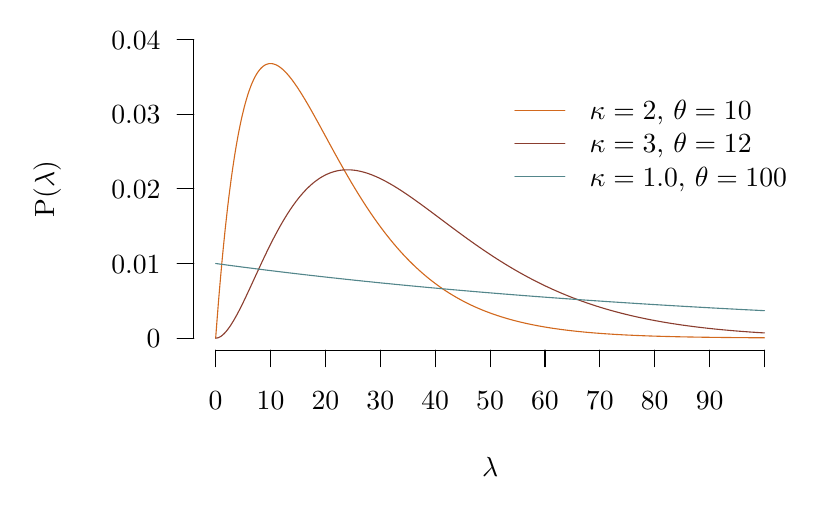
\begin{tikzpicture}[x=1pt,y=1pt]
\definecolor{fillColor}{RGB}{255,255,255}
\path[use as bounding box,fill=fillColor,fill opacity=0.00] (0,0) rectangle (274.17,164.50);
\begin{scope}
\path[clip] ( 60.00, 48.00) rectangle (274.17,164.50);
\definecolor{drawColor}{RGB}{210,105,30}

\path[draw=drawColor,line width= 0.4pt,line join=round,line cap=round] ( 67.93, 52.31) --
	( 68.13, 54.98) --
	( 68.33, 57.60) --
	( 68.53, 60.17) --
	( 68.73, 62.68) --
	( 68.92, 65.14) --
	( 69.12, 67.55) --
	( 69.32, 69.92) --
	( 69.52, 72.23) --
	( 69.72, 74.50) --
	( 69.92, 76.72) --
	( 70.11, 78.89) --
	( 70.31, 81.02) --
	( 70.51, 83.10) --
	( 70.71, 85.14) --
	( 70.91, 87.13) --
	( 71.11, 89.08) --
	( 71.30, 90.99) --
	( 71.50, 92.86) --
	( 71.70, 94.69) --
	( 71.90, 96.47) --
	( 72.10, 98.22) --
	( 72.29, 99.93) --
	( 72.49,101.60) --
	( 72.69,103.23) --
	( 72.89,104.82) --
	( 73.09,106.38) --
	( 73.29,107.90) --
	( 73.48,109.38) --
	( 73.68,110.83) --
	( 73.88,112.25) --
	( 74.08,113.63) --
	( 74.28,114.98) --
	( 74.48,116.30) --
	( 74.67,117.58) --
	( 74.87,118.83) --
	( 75.07,120.05) --
	( 75.27,121.24) --
	( 75.47,122.40) --
	( 75.67,123.52) --
	( 75.86,124.62) --
	( 76.06,125.69) --
	( 76.26,126.74) --
	( 76.46,127.75) --
	( 76.66,128.74) --
	( 76.86,129.70) --
	( 77.05,130.63) --
	( 77.25,131.53) --
	( 77.45,132.41) --
	( 77.65,133.27) --
	( 77.85,134.10) --
	( 78.05,134.91) --
	( 78.24,135.69) --
	( 78.44,136.45) --
	( 78.64,137.18) --
	( 78.84,137.89) --
	( 79.04,138.58) --
	( 79.24,139.25) --
	( 79.43,139.89) --
	( 79.63,140.52) --
	( 79.83,141.12) --
	( 80.03,141.70) --
	( 80.23,142.26) --
	( 80.43,142.80) --
	( 80.62,143.32) --
	( 80.82,143.83) --
	( 81.02,144.31) --
	( 81.22,144.77) --
	( 81.42,145.22) --
	( 81.62,145.65) --
	( 81.81,146.06) --
	( 82.01,146.45) --
	( 82.21,146.83) --
	( 82.41,147.19) --
	( 82.61,147.53) --
	( 82.81,147.86) --
	( 83.00,148.17) --
	( 83.20,148.46) --
	( 83.40,148.74) --
	( 83.60,149.01) --
	( 83.80,149.26) --
	( 84.00,149.49) --
	( 84.19,149.71) --
	( 84.39,149.92) --
	( 84.59,150.11) --
	( 84.79,150.29) --
	( 84.99,150.46) --
	( 85.18,150.61) --
	( 85.38,150.75) --
	( 85.58,150.88) --
	( 85.78,150.99) --
	( 85.98,151.10) --
	( 86.18,151.19) --
	( 86.37,151.27) --
	( 86.57,151.34) --
	( 86.77,151.40) --
	( 86.97,151.44) --
	( 87.17,151.48) --
	( 87.37,151.51) --
	( 87.56,151.52) --
	( 87.76,151.53) --
	( 87.96,151.52) --
	( 88.16,151.51) --
	( 88.36,151.48) --
	( 88.56,151.45) --
	( 88.75,151.41) --
	( 88.95,151.35) --
	( 89.15,151.29) --
	( 89.35,151.22) --
	( 89.55,151.15) --
	( 89.75,151.06) --
	( 89.94,150.97) --
	( 90.14,150.87) --
	( 90.34,150.76) --
	( 90.54,150.64) --
	( 90.74,150.51) --
	( 90.94,150.38) --
	( 91.13,150.24) --
	( 91.33,150.10) --
	( 91.53,149.95) --
	( 91.73,149.79) --
	( 91.93,149.62) --
	( 92.13,149.45) --
	( 92.32,149.27) --
	( 92.52,149.09) --
	( 92.72,148.90) --
	( 92.92,148.70) --
	( 93.12,148.50) --
	( 93.32,148.29) --
	( 93.51,148.08) --
	( 93.71,147.86) --
	( 93.91,147.64) --
	( 94.11,147.41) --
	( 94.31,147.18) --
	( 94.51,146.94) --
	( 94.70,146.70) --
	( 94.90,146.45) --
	( 95.10,146.20) --
	( 95.30,145.94) --
	( 95.50,145.68) --
	( 95.70,145.42) --
	( 95.89,145.15) --
	( 96.09,144.88) --
	( 96.29,144.60) --
	( 96.49,144.32) --
	( 96.69,144.04) --
	( 96.88,143.75) --
	( 97.08,143.46) --
	( 97.28,143.17) --
	( 97.48,142.88) --
	( 97.68,142.58) --
	( 97.88,142.27) --
	( 98.07,141.97) --
	( 98.27,141.66) --
	( 98.47,141.35) --
	( 98.67,141.04) --
	( 98.87,140.72) --
	( 99.07,140.40) --
	( 99.26,140.08) --
	( 99.46,139.76) --
	( 99.66,139.43) --
	( 99.86,139.10) --
	(100.06,138.77) --
	(100.26,138.44) --
	(100.45,138.11) --
	(100.65,137.77) --
	(100.85,137.43) --
	(101.05,137.10) --
	(101.25,136.75) --
	(101.45,136.41) --
	(101.64,136.07) --
	(101.84,135.72) --
	(102.04,135.38) --
	(102.24,135.03) --
	(102.44,134.68) --
	(102.64,134.33) --
	(102.83,133.97) --
	(103.03,133.62) --
	(103.23,133.27) --
	(103.43,132.91) --
	(103.63,132.56) --
	(103.83,132.20) --
	(104.02,131.84) --
	(104.22,131.48) --
	(104.42,131.12) --
	(104.62,130.76) --
	(104.82,130.40) --
	(105.02,130.04) --
	(105.21,129.68) --
	(105.41,129.32) --
	(105.61,128.95) --
	(105.81,128.59) --
	(106.01,128.23) --
	(106.21,127.86) --
	(106.40,127.50) --
	(106.60,127.13) --
	(106.80,126.77) --
	(107.00,126.40) --
	(107.20,126.04) --
	(107.40,125.67) --
	(107.59,125.31) --
	(107.79,124.94) --
	(107.99,124.58) --
	(108.19,124.22) --
	(108.39,123.85) --
	(108.59,123.49) --
	(108.78,123.12) --
	(108.98,122.76) --
	(109.18,122.39) --
	(109.38,122.03) --
	(109.58,121.67) --
	(109.77,121.30) --
	(109.97,120.94) --
	(110.17,120.58) --
	(110.37,120.22) --
	(110.57,119.85) --
	(110.77,119.49) --
	(110.96,119.13) --
	(111.16,118.77) --
	(111.36,118.41) --
	(111.56,118.05) --
	(111.76,117.70) --
	(111.96,117.34) --
	(112.15,116.98) --
	(112.35,116.63) --
	(112.55,116.27) --
	(112.75,115.91) --
	(112.95,115.56) --
	(113.15,115.21) --
	(113.34,114.85) --
	(113.54,114.50) --
	(113.74,114.15) --
	(113.94,113.80) --
	(114.14,113.45) --
	(114.34,113.10) --
	(114.53,112.76) --
	(114.73,112.41) --
	(114.93,112.06) --
	(115.13,111.72) --
	(115.33,111.37) --
	(115.53,111.03) --
	(115.72,110.69) --
	(115.92,110.35) --
	(116.12,110.01) --
	(116.32,109.67) --
	(116.52,109.33) --
	(116.72,108.99) --
	(116.91,108.66) --
	(117.11,108.32) --
	(117.31,107.99) --
	(117.51,107.66) --
	(117.71,107.33) --
	(117.91,107.00) --
	(118.10,106.67) --
	(118.30,106.34) --
	(118.50,106.01) --
	(118.70,105.68) --
	(118.90,105.36) --
	(119.10,105.04) --
	(119.29,104.71) --
	(119.49,104.39) --
	(119.69,104.07) --
	(119.89,103.75) --
	(120.09,103.44) --
	(120.29,103.12) --
	(120.48,102.81) --
	(120.68,102.49) --
	(120.88,102.18) --
	(121.08,101.87) --
	(121.28,101.56) --
	(121.47,101.25) --
	(121.67,100.94) --
	(121.87,100.64) --
	(122.07,100.33) --
	(122.27,100.03) --
	(122.47, 99.73) --
	(122.66, 99.42) --
	(122.86, 99.12) --
	(123.06, 98.83) --
	(123.26, 98.53) --
	(123.46, 98.23) --
	(123.66, 97.94) --
	(123.85, 97.65) --
	(124.05, 97.35) --
	(124.25, 97.06) --
	(124.45, 96.77) --
	(124.65, 96.49) --
	(124.85, 96.20) --
	(125.04, 95.91) --
	(125.24, 95.63) --
	(125.44, 95.35) --
	(125.64, 95.07) --
	(125.84, 94.79) --
	(126.04, 94.51) --
	(126.23, 94.23) --
	(126.43, 93.95) --
	(126.63, 93.68) --
	(126.83, 93.41) --
	(127.03, 93.13) --
	(127.23, 92.86) --
	(127.42, 92.59) --
	(127.62, 92.33) --
	(127.82, 92.06) --
	(128.02, 91.80) --
	(128.22, 91.53) --
	(128.42, 91.27) --
	(128.61, 91.01) --
	(128.81, 90.75) --
	(129.01, 90.49) --
	(129.21, 90.23) --
	(129.41, 89.98) --
	(129.61, 89.72) --
	(129.80, 89.47) --
	(130.00, 89.22) --
	(130.20, 88.97) --
	(130.40, 88.72) --
	(130.60, 88.47) --
	(130.80, 88.22) --
	(130.99, 87.98) --
	(131.19, 87.73) --
	(131.39, 87.49) --
	(131.59, 87.25) --
	(131.79, 87.01) --
	(131.99, 86.77) --
	(132.18, 86.54) --
	(132.38, 86.30) --
	(132.58, 86.06) --
	(132.78, 85.83) --
	(132.98, 85.60) --
	(133.18, 85.37) --
	(133.37, 85.14) --
	(133.57, 84.91) --
	(133.77, 84.68) --
	(133.97, 84.46) --
	(134.17, 84.23) --
	(134.36, 84.01) --
	(134.56, 83.79) --
	(134.76, 83.57) --
	(134.96, 83.35) --
	(135.16, 83.13) --
	(135.36, 82.92) --
	(135.55, 82.70) --
	(135.75, 82.49) --
	(135.95, 82.27) --
	(136.15, 82.06) --
	(136.35, 81.85) --
	(136.55, 81.64) --
	(136.74, 81.43) --
	(136.94, 81.23) --
	(137.14, 81.02) --
	(137.34, 80.82) --
	(137.54, 80.61) --
	(137.74, 80.41) --
	(137.93, 80.21) --
	(138.13, 80.01) --
	(138.33, 79.82) --
	(138.53, 79.62) --
	(138.73, 79.42) --
	(138.93, 79.23) --
	(139.12, 79.03) --
	(139.32, 78.84) --
	(139.52, 78.65) --
	(139.72, 78.46) --
	(139.92, 78.27) --
	(140.12, 78.09) --
	(140.31, 77.90) --
	(140.51, 77.71) --
	(140.71, 77.53) --
	(140.91, 77.35) --
	(141.11, 77.17) --
	(141.31, 76.98) --
	(141.50, 76.81) --
	(141.70, 76.63) --
	(141.90, 76.45) --
	(142.10, 76.27) --
	(142.30, 76.10) --
	(142.50, 75.92) --
	(142.69, 75.75) --
	(142.89, 75.58) --
	(143.09, 75.41) --
	(143.29, 75.24) --
	(143.49, 75.07) --
	(143.69, 74.90) --
	(143.88, 74.74) --
	(144.08, 74.57) --
	(144.28, 74.41) --
	(144.48, 74.25) --
	(144.68, 74.08) --
	(144.88, 73.92) --
	(145.07, 73.76) --
	(145.27, 73.60) --
	(145.47, 73.45) --
	(145.67, 73.29) --
	(145.87, 73.13) --
	(146.06, 72.98) --
	(146.26, 72.83) --
	(146.46, 72.67) --
	(146.66, 72.52) --
	(146.86, 72.37) --
	(147.06, 72.22) --
	(147.25, 72.07) --
	(147.45, 71.92) --
	(147.65, 71.78) --
	(147.85, 71.63) --
	(148.05, 71.49) --
	(148.25, 71.34) --
	(148.44, 71.20) --
	(148.64, 71.06) --
	(148.84, 70.92) --
	(149.04, 70.78) --
	(149.24, 70.64) --
	(149.44, 70.50) --
	(149.63, 70.36) --
	(149.83, 70.23) --
	(150.03, 70.09) --
	(150.23, 69.96) --
	(150.43, 69.82) --
	(150.63, 69.69) --
	(150.82, 69.56) --
	(151.02, 69.43) --
	(151.22, 69.30) --
	(151.42, 69.17) --
	(151.62, 69.04) --
	(151.82, 68.92) --
	(152.01, 68.79) --
	(152.21, 68.66) --
	(152.41, 68.54) --
	(152.61, 68.42) --
	(152.81, 68.29) --
	(153.01, 68.17) --
	(153.20, 68.05) --
	(153.40, 67.93) --
	(153.60, 67.81) --
	(153.80, 67.69) --
	(154.00, 67.57) --
	(154.20, 67.46) --
	(154.39, 67.34) --
	(154.59, 67.22) --
	(154.79, 67.11) --
	(154.99, 67.00) --
	(155.19, 66.88) --
	(155.39, 66.77) --
	(155.58, 66.66) --
	(155.78, 66.55) --
	(155.98, 66.44) --
	(156.18, 66.33) --
	(156.38, 66.22) --
	(156.58, 66.11) --
	(156.77, 66.01) --
	(156.97, 65.90) --
	(157.17, 65.80) --
	(157.37, 65.69) --
	(157.57, 65.59) --
	(157.77, 65.49) --
	(157.96, 65.38) --
	(158.16, 65.28) --
	(158.36, 65.18) --
	(158.56, 65.08) --
	(158.76, 64.98) --
	(158.95, 64.88) --
	(159.15, 64.78) --
	(159.35, 64.69) --
	(159.55, 64.59) --
	(159.75, 64.49) --
	(159.95, 64.40) --
	(160.14, 64.31) --
	(160.34, 64.21) --
	(160.54, 64.12) --
	(160.74, 64.03) --
	(160.94, 63.93) --
	(161.14, 63.84) --
	(161.33, 63.75) --
	(161.53, 63.66) --
	(161.73, 63.57) --
	(161.93, 63.49) --
	(162.13, 63.40) --
	(162.33, 63.31) --
	(162.52, 63.22) --
	(162.72, 63.14) --
	(162.92, 63.05) --
	(163.12, 62.97) --
	(163.32, 62.88) --
	(163.52, 62.80) --
	(163.71, 62.72) --
	(163.91, 62.64) --
	(164.11, 62.55) --
	(164.31, 62.47) --
	(164.51, 62.39) --
	(164.71, 62.31) --
	(164.90, 62.23) --
	(165.10, 62.16) --
	(165.30, 62.08) --
	(165.50, 62.00) --
	(165.70, 61.92) --
	(165.90, 61.85) --
	(166.09, 61.77) --
	(166.29, 61.70) --
	(166.49, 61.62) --
	(166.69, 61.55) --
	(166.89, 61.47) --
	(167.09, 61.40) --
	(167.28, 61.33) --
	(167.48, 61.26) --
	(167.68, 61.18) --
	(167.88, 61.11) --
	(168.08, 61.04) --
	(168.28, 60.97) --
	(168.47, 60.90) --
	(168.67, 60.84) --
	(168.87, 60.77) --
	(169.07, 60.70) --
	(169.27, 60.63) --
	(169.47, 60.57) --
	(169.66, 60.50) --
	(169.86, 60.43) --
	(170.06, 60.37) --
	(170.26, 60.30) --
	(170.46, 60.24) --
	(170.65, 60.18) --
	(170.85, 60.11) --
	(171.05, 60.05) --
	(171.25, 59.99) --
	(171.45, 59.93) --
	(171.65, 59.87) --
	(171.84, 59.80) --
	(172.04, 59.74) --
	(172.24, 59.68) --
	(172.44, 59.63) --
	(172.64, 59.57) --
	(172.84, 59.51) --
	(173.03, 59.45) --
	(173.23, 59.39) --
	(173.43, 59.33) --
	(173.63, 59.28) --
	(173.83, 59.22) --
	(174.03, 59.17) --
	(174.22, 59.11) --
	(174.42, 59.05) --
	(174.62, 59.00) --
	(174.82, 58.95) --
	(175.02, 58.89) --
	(175.22, 58.84) --
	(175.41, 58.79) --
	(175.61, 58.73) --
	(175.81, 58.68) --
	(176.01, 58.63) --
	(176.21, 58.58) --
	(176.41, 58.53) --
	(176.60, 58.48) --
	(176.80, 58.43) --
	(177.00, 58.38) --
	(177.20, 58.33) --
	(177.40, 58.28) --
	(177.60, 58.23) --
	(177.79, 58.18) --
	(177.99, 58.13) --
	(178.19, 58.09) --
	(178.39, 58.04) --
	(178.59, 57.99) --
	(178.79, 57.95) --
	(178.98, 57.90) --
	(179.18, 57.85) --
	(179.38, 57.81) --
	(179.58, 57.76) --
	(179.78, 57.72) --
	(179.98, 57.67) --
	(180.17, 57.63) --
	(180.37, 57.59) --
	(180.57, 57.54) --
	(180.77, 57.50) --
	(180.97, 57.46) --
	(181.17, 57.42) --
	(181.36, 57.37) --
	(181.56, 57.33) --
	(181.76, 57.29) --
	(181.96, 57.25) --
	(182.16, 57.21) --
	(182.35, 57.17) --
	(182.55, 57.13) --
	(182.75, 57.09) --
	(182.95, 57.05) --
	(183.15, 57.01) --
	(183.35, 56.97) --
	(183.54, 56.93) --
	(183.74, 56.90) --
	(183.94, 56.86) --
	(184.14, 56.82) --
	(184.34, 56.78) --
	(184.54, 56.75) --
	(184.73, 56.71) --
	(184.93, 56.67) --
	(185.13, 56.64) --
	(185.33, 56.60) --
	(185.53, 56.57) --
	(185.73, 56.53) --
	(185.92, 56.50) --
	(186.12, 56.46) --
	(186.32, 56.43) --
	(186.52, 56.39) --
	(186.72, 56.36) --
	(186.92, 56.33) --
	(187.11, 56.29) --
	(187.31, 56.26) --
	(187.51, 56.23) --
	(187.71, 56.19) --
	(187.91, 56.16) --
	(188.11, 56.13) --
	(188.30, 56.10) --
	(188.50, 56.07) --
	(188.70, 56.04) --
	(188.90, 56.00) --
	(189.10, 55.97) --
	(189.30, 55.94) --
	(189.49, 55.91) --
	(189.69, 55.88) --
	(189.89, 55.85) --
	(190.09, 55.82) --
	(190.29, 55.79) --
	(190.49, 55.77) --
	(190.68, 55.74) --
	(190.88, 55.71) --
	(191.08, 55.68) --
	(191.28, 55.65) --
	(191.48, 55.62) --
	(191.68, 55.60) --
	(191.87, 55.57) --
	(192.07, 55.54) --
	(192.27, 55.51) --
	(192.47, 55.49) --
	(192.67, 55.46) --
	(192.87, 55.43) --
	(193.06, 55.41) --
	(193.26, 55.38) --
	(193.46, 55.36) --
	(193.66, 55.33) --
	(193.86, 55.31) --
	(194.06, 55.28) --
	(194.25, 55.26) --
	(194.45, 55.23) --
	(194.65, 55.21) --
	(194.85, 55.18) --
	(195.05, 55.16) --
	(195.24, 55.13) --
	(195.44, 55.11) --
	(195.64, 55.09) --
	(195.84, 55.06) --
	(196.04, 55.04) --
	(196.24, 55.02) --
	(196.43, 55.00) --
	(196.63, 54.97) --
	(196.83, 54.95) --
	(197.03, 54.93) --
	(197.23, 54.91) --
	(197.43, 54.88) --
	(197.62, 54.86) --
	(197.82, 54.84) --
	(198.02, 54.82) --
	(198.22, 54.80) --
	(198.42, 54.78) --
	(198.62, 54.76) --
	(198.81, 54.74) --
	(199.01, 54.72) --
	(199.21, 54.70) --
	(199.41, 54.68) --
	(199.61, 54.66) --
	(199.81, 54.64) --
	(200.00, 54.62) --
	(200.20, 54.60) --
	(200.40, 54.58) --
	(200.60, 54.56) --
	(200.80, 54.54) --
	(201.00, 54.52) --
	(201.19, 54.50) --
	(201.39, 54.48) --
	(201.59, 54.46) --
	(201.79, 54.45) --
	(201.99, 54.43) --
	(202.19, 54.41) --
	(202.38, 54.39) --
	(202.58, 54.37) --
	(202.78, 54.36) --
	(202.98, 54.34) --
	(203.18, 54.32) --
	(203.38, 54.31) --
	(203.57, 54.29) --
	(203.77, 54.27) --
	(203.97, 54.26) --
	(204.17, 54.24) --
	(204.37, 54.22) --
	(204.57, 54.21) --
	(204.76, 54.19) --
	(204.96, 54.17) --
	(205.16, 54.16) --
	(205.36, 54.14) --
	(205.56, 54.13) --
	(205.76, 54.11) --
	(205.95, 54.10) --
	(206.15, 54.08) --
	(206.35, 54.07) --
	(206.55, 54.05) --
	(206.75, 54.04) --
	(206.94, 54.02) --
	(207.14, 54.01) --
	(207.34, 53.99) --
	(207.54, 53.98) --
	(207.74, 53.96) --
	(207.94, 53.95) --
	(208.13, 53.94) --
	(208.33, 53.92) --
	(208.53, 53.91) --
	(208.73, 53.89) --
	(208.93, 53.88) --
	(209.13, 53.87) --
	(209.32, 53.85) --
	(209.52, 53.84) --
	(209.72, 53.83) --
	(209.92, 53.82) --
	(210.12, 53.80) --
	(210.32, 53.79) --
	(210.51, 53.78) --
	(210.71, 53.76) --
	(210.91, 53.75) --
	(211.11, 53.74) --
	(211.31, 53.73) --
	(211.51, 53.72) --
	(211.70, 53.70) --
	(211.90, 53.69) --
	(212.10, 53.68) --
	(212.30, 53.67) --
	(212.50, 53.66) --
	(212.70, 53.64) --
	(212.89, 53.63) --
	(213.09, 53.62) --
	(213.29, 53.61) --
	(213.49, 53.60) --
	(213.69, 53.59) --
	(213.89, 53.58) --
	(214.08, 53.57) --
	(214.28, 53.56) --
	(214.48, 53.55) --
	(214.68, 53.53) --
	(214.88, 53.52) --
	(215.08, 53.51) --
	(215.27, 53.50) --
	(215.47, 53.49) --
	(215.67, 53.48) --
	(215.87, 53.47) --
	(216.07, 53.46) --
	(216.27, 53.45) --
	(216.46, 53.44) --
	(216.66, 53.43) --
	(216.86, 53.42) --
	(217.06, 53.41) --
	(217.26, 53.40) --
	(217.46, 53.40) --
	(217.65, 53.39) --
	(217.85, 53.38) --
	(218.05, 53.37) --
	(218.25, 53.36) --
	(218.45, 53.35) --
	(218.65, 53.34) --
	(218.84, 53.33) --
	(219.04, 53.32) --
	(219.24, 53.31) --
	(219.44, 53.31) --
	(219.64, 53.30) --
	(219.83, 53.29) --
	(220.03, 53.28) --
	(220.23, 53.27) --
	(220.43, 53.26) --
	(220.63, 53.26) --
	(220.83, 53.25) --
	(221.02, 53.24) --
	(221.22, 53.23) --
	(221.42, 53.22) --
	(221.62, 53.22) --
	(221.82, 53.21) --
	(222.02, 53.20) --
	(222.21, 53.19) --
	(222.41, 53.18) --
	(222.61, 53.18) --
	(222.81, 53.17) --
	(223.01, 53.16) --
	(223.21, 53.15) --
	(223.40, 53.15) --
	(223.60, 53.14) --
	(223.80, 53.13) --
	(224.00, 53.13) --
	(224.20, 53.12) --
	(224.40, 53.11) --
	(224.59, 53.10) --
	(224.79, 53.10) --
	(224.99, 53.09) --
	(225.19, 53.08) --
	(225.39, 53.08) --
	(225.59, 53.07) --
	(225.78, 53.06) --
	(225.98, 53.06) --
	(226.18, 53.05) --
	(226.38, 53.05) --
	(226.58, 53.04) --
	(226.78, 53.03) --
	(226.97, 53.03) --
	(227.17, 53.02) --
	(227.37, 53.01) --
	(227.57, 53.01) --
	(227.77, 53.00) --
	(227.97, 53.00) --
	(228.16, 52.99) --
	(228.36, 52.98) --
	(228.56, 52.98) --
	(228.76, 52.97) --
	(228.96, 52.97) --
	(229.16, 52.96) --
	(229.35, 52.96) --
	(229.55, 52.95) --
	(229.75, 52.94) --
	(229.95, 52.94) --
	(230.15, 52.93) --
	(230.35, 52.93) --
	(230.54, 52.92) --
	(230.74, 52.92) --
	(230.94, 52.91) --
	(231.14, 52.91) --
	(231.34, 52.90) --
	(231.53, 52.90) --
	(231.73, 52.89) --
	(231.93, 52.89) --
	(232.13, 52.88) --
	(232.33, 52.88) --
	(232.53, 52.87) --
	(232.72, 52.87) --
	(232.92, 52.86) --
	(233.12, 52.86) --
	(233.32, 52.85) --
	(233.52, 52.85) --
	(233.72, 52.84) --
	(233.91, 52.84) --
	(234.11, 52.83) --
	(234.31, 52.83) --
	(234.51, 52.82) --
	(234.71, 52.82) --
	(234.91, 52.82) --
	(235.10, 52.81) --
	(235.30, 52.81) --
	(235.50, 52.80) --
	(235.70, 52.80) --
	(235.90, 52.79) --
	(236.10, 52.79) --
	(236.29, 52.79) --
	(236.49, 52.78) --
	(236.69, 52.78) --
	(236.89, 52.77) --
	(237.09, 52.77) --
	(237.29, 52.77) --
	(237.48, 52.76) --
	(237.68, 52.76) --
	(237.88, 52.75) --
	(238.08, 52.75) --
	(238.28, 52.75) --
	(238.48, 52.74) --
	(238.67, 52.74) --
	(238.87, 52.73) --
	(239.07, 52.73) --
	(239.27, 52.73) --
	(239.47, 52.72) --
	(239.67, 52.72) --
	(239.86, 52.72) --
	(240.06, 52.71) --
	(240.26, 52.71) --
	(240.46, 52.71) --
	(240.66, 52.70) --
	(240.86, 52.70) --
	(241.05, 52.70) --
	(241.25, 52.69) --
	(241.45, 52.69) --
	(241.65, 52.69) --
	(241.85, 52.68) --
	(242.05, 52.68) --
	(242.24, 52.68) --
	(242.44, 52.67) --
	(242.64, 52.67) --
	(242.84, 52.67) --
	(243.04, 52.66) --
	(243.24, 52.66) --
	(243.43, 52.66) --
	(243.63, 52.65) --
	(243.83, 52.65) --
	(244.03, 52.65) --
	(244.23, 52.65) --
	(244.42, 52.64) --
	(244.62, 52.64) --
	(244.82, 52.64) --
	(245.02, 52.63) --
	(245.22, 52.63) --
	(245.42, 52.63) --
	(245.61, 52.63) --
	(245.81, 52.62) --
	(246.01, 52.62) --
	(246.21, 52.62) --
	(246.41, 52.61) --
	(246.61, 52.61) --
	(246.80, 52.61) --
	(247.00, 52.61) --
	(247.20, 52.60) --
	(247.40, 52.60) --
	(247.60, 52.60) --
	(247.80, 52.60) --
	(247.99, 52.59) --
	(248.19, 52.59) --
	(248.39, 52.59) --
	(248.59, 52.59) --
	(248.79, 52.58) --
	(248.99, 52.58) --
	(249.18, 52.58) --
	(249.38, 52.58) --
	(249.58, 52.57) --
	(249.78, 52.57) --
	(249.98, 52.57) --
	(250.18, 52.57) --
	(250.37, 52.57) --
	(250.57, 52.56) --
	(250.77, 52.56) --
	(250.97, 52.56) --
	(251.17, 52.56) --
	(251.37, 52.55) --
	(251.56, 52.55) --
	(251.76, 52.55) --
	(251.96, 52.55) --
	(252.16, 52.55) --
	(252.36, 52.54) --
	(252.56, 52.54) --
	(252.75, 52.54) --
	(252.95, 52.54) --
	(253.15, 52.54) --
	(253.35, 52.53) --
	(253.55, 52.53) --
	(253.75, 52.53) --
	(253.94, 52.53) --
	(254.14, 52.53) --
	(254.34, 52.52) --
	(254.54, 52.52) --
	(254.74, 52.52) --
	(254.94, 52.52) --
	(255.13, 52.52) --
	(255.33, 52.52) --
	(255.53, 52.51) --
	(255.73, 52.51) --
	(255.93, 52.51) --
	(256.12, 52.51) --
	(256.32, 52.51) --
	(256.52, 52.50) --
	(256.72, 52.50) --
	(256.92, 52.50) --
	(257.12, 52.50) --
	(257.31, 52.50) --
	(257.51, 52.50) --
	(257.71, 52.50) --
	(257.91, 52.49) --
	(258.11, 52.49) --
	(258.31, 52.49) --
	(258.50, 52.49) --
	(258.70, 52.49) --
	(258.90, 52.49) --
	(259.10, 52.48) --
	(259.30, 52.48) --
	(259.50, 52.48) --
	(259.69, 52.48) --
	(259.89, 52.48) --
	(260.09, 52.48) --
	(260.29, 52.48) --
	(260.49, 52.47) --
	(260.69, 52.47) --
	(260.88, 52.47) --
	(261.08, 52.47) --
	(261.28, 52.47) --
	(261.48, 52.47) --
	(261.68, 52.47) --
	(261.88, 52.46) --
	(262.07, 52.46) --
	(262.27, 52.46) --
	(262.47, 52.46) --
	(262.67, 52.46) --
	(262.87, 52.46) --
	(263.07, 52.46) --
	(263.26, 52.46) --
	(263.46, 52.45) --
	(263.66, 52.45) --
	(263.86, 52.45) --
	(264.06, 52.45) --
	(264.26, 52.45) --
	(264.45, 52.45) --
	(264.65, 52.45) --
	(264.85, 52.45) --
	(265.05, 52.44) --
	(265.25, 52.44) --
	(265.45, 52.44) --
	(265.64, 52.44) --
	(265.84, 52.44) --
	(266.04, 52.44) --
	(266.24, 52.44);
\end{scope}
\begin{scope}
\path[clip] ( 60.00, 48.00) rectangle (274.17,164.50);
\definecolor{drawColor}{RGB}{139,62,47}

\path[draw=drawColor,line width= 0.4pt,line join=round,line cap=round] ( 67.93, 52.31) --
	( 68.13, 52.32) --
	( 68.33, 52.35) --
	( 68.53, 52.38) --
	( 68.73, 52.44) --
	( 68.92, 52.50) --
	( 69.12, 52.58) --
	( 69.32, 52.68) --
	( 69.52, 52.78) --
	( 69.72, 52.90) --
	( 69.92, 53.03) --
	( 70.11, 53.18) --
	( 70.31, 53.33) --
	( 70.51, 53.50) --
	( 70.71, 53.68) --
	( 70.91, 53.86) --
	( 71.11, 54.06) --
	( 71.30, 54.27) --
	( 71.50, 54.49) --
	( 71.70, 54.72) --
	( 71.90, 54.96) --
	( 72.10, 55.20) --
	( 72.29, 55.46) --
	( 72.49, 55.72) --
	( 72.69, 55.99) --
	( 72.89, 56.27) --
	( 73.09, 56.56) --
	( 73.29, 56.86) --
	( 73.48, 57.16) --
	( 73.68, 57.47) --
	( 73.88, 57.78) --
	( 74.08, 58.11) --
	( 74.28, 58.44) --
	( 74.48, 58.77) --
	( 74.67, 59.11) --
	( 74.87, 59.46) --
	( 75.07, 59.81) --
	( 75.27, 60.16) --
	( 75.47, 60.52) --
	( 75.67, 60.89) --
	( 75.86, 61.26) --
	( 76.06, 61.64) --
	( 76.26, 62.01) --
	( 76.46, 62.40) --
	( 76.66, 62.78) --
	( 76.86, 63.18) --
	( 77.05, 63.57) --
	( 77.25, 63.97) --
	( 77.45, 64.37) --
	( 77.65, 64.77) --
	( 77.85, 65.18) --
	( 78.05, 65.58) --
	( 78.24, 66.00) --
	( 78.44, 66.41) --
	( 78.64, 66.82) --
	( 78.84, 67.24) --
	( 79.04, 67.66) --
	( 79.24, 68.08) --
	( 79.43, 68.50) --
	( 79.63, 68.93) --
	( 79.83, 69.35) --
	( 80.03, 69.78) --
	( 80.23, 70.21) --
	( 80.43, 70.64) --
	( 80.62, 71.07) --
	( 80.82, 71.50) --
	( 81.02, 71.93) --
	( 81.22, 72.36) --
	( 81.42, 72.79) --
	( 81.62, 73.22) --
	( 81.81, 73.65) --
	( 82.01, 74.08) --
	( 82.21, 74.52) --
	( 82.41, 74.95) --
	( 82.61, 75.38) --
	( 82.81, 75.81) --
	( 83.00, 76.24) --
	( 83.20, 76.67) --
	( 83.40, 77.10) --
	( 83.60, 77.53) --
	( 83.80, 77.96) --
	( 84.00, 78.38) --
	( 84.19, 78.81) --
	( 84.39, 79.23) --
	( 84.59, 79.66) --
	( 84.79, 80.08) --
	( 84.99, 80.50) --
	( 85.18, 80.92) --
	( 85.38, 81.34) --
	( 85.58, 81.76) --
	( 85.78, 82.17) --
	( 85.98, 82.59) --
	( 86.18, 83.00) --
	( 86.37, 83.41) --
	( 86.57, 83.82) --
	( 86.77, 84.22) --
	( 86.97, 84.63) --
	( 87.17, 85.03) --
	( 87.37, 85.43) --
	( 87.56, 85.83) --
	( 87.76, 86.23) --
	( 87.96, 86.62) --
	( 88.16, 87.01) --
	( 88.36, 87.40) --
	( 88.56, 87.79) --
	( 88.75, 88.18) --
	( 88.95, 88.56) --
	( 89.15, 88.94) --
	( 89.35, 89.32) --
	( 89.55, 89.70) --
	( 89.75, 90.07) --
	( 89.94, 90.44) --
	( 90.14, 90.81) --
	( 90.34, 91.17) --
	( 90.54, 91.53) --
	( 90.74, 91.89) --
	( 90.94, 92.25) --
	( 91.13, 92.61) --
	( 91.33, 92.96) --
	( 91.53, 93.31) --
	( 91.73, 93.65) --
	( 91.93, 94.00) --
	( 92.13, 94.34) --
	( 92.32, 94.67) --
	( 92.52, 95.01) --
	( 92.72, 95.34) --
	( 92.92, 95.67) --
	( 93.12, 95.99) --
	( 93.32, 96.31) --
	( 93.51, 96.63) --
	( 93.71, 96.95) --
	( 93.91, 97.26) --
	( 94.11, 97.57) --
	( 94.31, 97.88) --
	( 94.51, 98.18) --
	( 94.70, 98.49) --
	( 94.90, 98.78) --
	( 95.10, 99.08) --
	( 95.30, 99.37) --
	( 95.50, 99.66) --
	( 95.70, 99.94) --
	( 95.89,100.22) --
	( 96.09,100.50) --
	( 96.29,100.78) --
	( 96.49,101.05) --
	( 96.69,101.32) --
	( 96.88,101.59) --
	( 97.08,101.85) --
	( 97.28,102.11) --
	( 97.48,102.36) --
	( 97.68,102.62) --
	( 97.88,102.87) --
	( 98.07,103.11) --
	( 98.27,103.36) --
	( 98.47,103.60) --
	( 98.67,103.84) --
	( 98.87,104.07) --
	( 99.07,104.30) --
	( 99.26,104.53) --
	( 99.46,104.75) --
	( 99.66,104.97) --
	( 99.86,105.19) --
	(100.06,105.40) --
	(100.26,105.62) --
	(100.45,105.82) --
	(100.65,106.03) --
	(100.85,106.23) --
	(101.05,106.43) --
	(101.25,106.63) --
	(101.45,106.82) --
	(101.64,107.01) --
	(101.84,107.19) --
	(102.04,107.38) --
	(102.24,107.56) --
	(102.44,107.73) --
	(102.64,107.91) --
	(102.83,108.08) --
	(103.03,108.24) --
	(103.23,108.41) --
	(103.43,108.57) --
	(103.63,108.73) --
	(103.83,108.88) --
	(104.02,109.04) --
	(104.22,109.18) --
	(104.42,109.33) --
	(104.62,109.47) --
	(104.82,109.61) --
	(105.02,109.75) --
	(105.21,109.89) --
	(105.41,110.02) --
	(105.61,110.14) --
	(105.81,110.27) --
	(106.01,110.39) --
	(106.21,110.51) --
	(106.40,110.63) --
	(106.60,110.74) --
	(106.80,110.85) --
	(107.00,110.96) --
	(107.20,111.07) --
	(107.40,111.17) --
	(107.59,111.27) --
	(107.79,111.37) --
	(107.99,111.46) --
	(108.19,111.55) --
	(108.39,111.64) --
	(108.59,111.73) --
	(108.78,111.81) --
	(108.98,111.89) --
	(109.18,111.97) --
	(109.38,112.04) --
	(109.58,112.11) --
	(109.77,112.18) --
	(109.97,112.25) --
	(110.17,112.32) --
	(110.37,112.38) --
	(110.57,112.44) --
	(110.77,112.50) --
	(110.96,112.55) --
	(111.16,112.60) --
	(111.36,112.65) --
	(111.56,112.70) --
	(111.76,112.74) --
	(111.96,112.78) --
	(112.15,112.82) --
	(112.35,112.86) --
	(112.55,112.90) --
	(112.75,112.93) --
	(112.95,112.96) --
	(113.15,112.99) --
	(113.34,113.01) --
	(113.54,113.04) --
	(113.74,113.06) --
	(113.94,113.07) --
	(114.14,113.09) --
	(114.34,113.11) --
	(114.53,113.12) --
	(114.73,113.13) --
	(114.93,113.13) --
	(115.13,113.14) --
	(115.33,113.14) --
	(115.53,113.14) --
	(115.72,113.14) --
	(115.92,113.14) --
	(116.12,113.13) --
	(116.32,113.13) --
	(116.52,113.12) --
	(116.72,113.11) --
	(116.91,113.09) --
	(117.11,113.08) --
	(117.31,113.06) --
	(117.51,113.04) --
	(117.71,113.02) --
	(117.91,113.00) --
	(118.10,112.97) --
	(118.30,112.95) --
	(118.50,112.92) --
	(118.70,112.89) --
	(118.90,112.85) --
	(119.10,112.82) --
	(119.29,112.78) --
	(119.49,112.75) --
	(119.69,112.71) --
	(119.89,112.66) --
	(120.09,112.62) --
	(120.29,112.58) --
	(120.48,112.53) --
	(120.68,112.48) --
	(120.88,112.43) --
	(121.08,112.38) --
	(121.28,112.33) --
	(121.47,112.27) --
	(121.67,112.22) --
	(121.87,112.16) --
	(122.07,112.10) --
	(122.27,112.04) --
	(122.47,111.98) --
	(122.66,111.91) --
	(122.86,111.85) --
	(123.06,111.78) --
	(123.26,111.71) --
	(123.46,111.64) --
	(123.66,111.57) --
	(123.85,111.50) --
	(124.05,111.42) --
	(124.25,111.35) --
	(124.45,111.27) --
	(124.65,111.19) --
	(124.85,111.11) --
	(125.04,111.03) --
	(125.24,110.95) --
	(125.44,110.87) --
	(125.64,110.78) --
	(125.84,110.69) --
	(126.04,110.61) --
	(126.23,110.52) --
	(126.43,110.43) --
	(126.63,110.34) --
	(126.83,110.25) --
	(127.03,110.15) --
	(127.23,110.06) --
	(127.42,109.96) --
	(127.62,109.87) --
	(127.82,109.77) --
	(128.02,109.67) --
	(128.22,109.57) --
	(128.42,109.47) --
	(128.61,109.37) --
	(128.81,109.26) --
	(129.01,109.16) --
	(129.21,109.05) --
	(129.41,108.95) --
	(129.61,108.84) --
	(129.80,108.73) --
	(130.00,108.62) --
	(130.20,108.51) --
	(130.40,108.40) --
	(130.60,108.29) --
	(130.80,108.18) --
	(130.99,108.07) --
	(131.19,107.95) --
	(131.39,107.84) --
	(131.59,107.72) --
	(131.79,107.60) --
	(131.99,107.49) --
	(132.18,107.37) --
	(132.38,107.25) --
	(132.58,107.13) --
	(132.78,107.01) --
	(132.98,106.88) --
	(133.18,106.76) --
	(133.37,106.64) --
	(133.57,106.52) --
	(133.77,106.39) --
	(133.97,106.27) --
	(134.17,106.14) --
	(134.36,106.01) --
	(134.56,105.89) --
	(134.76,105.76) --
	(134.96,105.63) --
	(135.16,105.50) --
	(135.36,105.37) --
	(135.55,105.24) --
	(135.75,105.11) --
	(135.95,104.98) --
	(136.15,104.85) --
	(136.35,104.71) --
	(136.55,104.58) --
	(136.74,104.45) --
	(136.94,104.31) --
	(137.14,104.18) --
	(137.34,104.04) --
	(137.54,103.91) --
	(137.74,103.77) --
	(137.93,103.63) --
	(138.13,103.50) --
	(138.33,103.36) --
	(138.53,103.22) --
	(138.73,103.08) --
	(138.93,102.94) --
	(139.12,102.80) --
	(139.32,102.66) --
	(139.52,102.52) --
	(139.72,102.38) --
	(139.92,102.24) --
	(140.12,102.10) --
	(140.31,101.96) --
	(140.51,101.82) --
	(140.71,101.68) --
	(140.91,101.53) --
	(141.11,101.39) --
	(141.31,101.25) --
	(141.50,101.11) --
	(141.70,100.96) --
	(141.90,100.82) --
	(142.10,100.67) --
	(142.30,100.53) --
	(142.50,100.38) --
	(142.69,100.24) --
	(142.89,100.09) --
	(143.09, 99.95) --
	(143.29, 99.80) --
	(143.49, 99.66) --
	(143.69, 99.51) --
	(143.88, 99.36) --
	(144.08, 99.22) --
	(144.28, 99.07) --
	(144.48, 98.92) --
	(144.68, 98.78) --
	(144.88, 98.63) --
	(145.07, 98.48) --
	(145.27, 98.34) --
	(145.47, 98.19) --
	(145.67, 98.04) --
	(145.87, 97.89) --
	(146.06, 97.74) --
	(146.26, 97.60) --
	(146.46, 97.45) --
	(146.66, 97.30) --
	(146.86, 97.15) --
	(147.06, 97.00) --
	(147.25, 96.85) --
	(147.45, 96.71) --
	(147.65, 96.56) --
	(147.85, 96.41) --
	(148.05, 96.26) --
	(148.25, 96.11) --
	(148.44, 95.96) --
	(148.64, 95.81) --
	(148.84, 95.67) --
	(149.04, 95.52) --
	(149.24, 95.37) --
	(149.44, 95.22) --
	(149.63, 95.07) --
	(149.83, 94.92) --
	(150.03, 94.77) --
	(150.23, 94.62) --
	(150.43, 94.48) --
	(150.63, 94.33) --
	(150.82, 94.18) --
	(151.02, 94.03) --
	(151.22, 93.88) --
	(151.42, 93.73) --
	(151.62, 93.58) --
	(151.82, 93.44) --
	(152.01, 93.29) --
	(152.21, 93.14) --
	(152.41, 92.99) --
	(152.61, 92.84) --
	(152.81, 92.70) --
	(153.01, 92.55) --
	(153.20, 92.40) --
	(153.40, 92.25) --
	(153.60, 92.11) --
	(153.80, 91.96) --
	(154.00, 91.81) --
	(154.20, 91.66) --
	(154.39, 91.52) --
	(154.59, 91.37) --
	(154.79, 91.22) --
	(154.99, 91.08) --
	(155.19, 90.93) --
	(155.39, 90.78) --
	(155.58, 90.64) --
	(155.78, 90.49) --
	(155.98, 90.35) --
	(156.18, 90.20) --
	(156.38, 90.06) --
	(156.58, 89.91) --
	(156.77, 89.77) --
	(156.97, 89.62) --
	(157.17, 89.48) --
	(157.37, 89.33) --
	(157.57, 89.19) --
	(157.77, 89.04) --
	(157.96, 88.90) --
	(158.16, 88.76) --
	(158.36, 88.61) --
	(158.56, 88.47) --
	(158.76, 88.33) --
	(158.95, 88.18) --
	(159.15, 88.04) --
	(159.35, 87.90) --
	(159.55, 87.76) --
	(159.75, 87.62) --
	(159.95, 87.47) --
	(160.14, 87.33) --
	(160.34, 87.19) --
	(160.54, 87.05) --
	(160.74, 86.91) --
	(160.94, 86.77) --
	(161.14, 86.63) --
	(161.33, 86.49) --
	(161.53, 86.35) --
	(161.73, 86.21) --
	(161.93, 86.07) --
	(162.13, 85.93) --
	(162.33, 85.80) --
	(162.52, 85.66) --
	(162.72, 85.52) --
	(162.92, 85.38) --
	(163.12, 85.24) --
	(163.32, 85.11) --
	(163.52, 84.97) --
	(163.71, 84.83) --
	(163.91, 84.70) --
	(164.11, 84.56) --
	(164.31, 84.43) --
	(164.51, 84.29) --
	(164.71, 84.16) --
	(164.90, 84.02) --
	(165.10, 83.89) --
	(165.30, 83.75) --
	(165.50, 83.62) --
	(165.70, 83.49) --
	(165.90, 83.35) --
	(166.09, 83.22) --
	(166.29, 83.09) --
	(166.49, 82.95) --
	(166.69, 82.82) --
	(166.89, 82.69) --
	(167.09, 82.56) --
	(167.28, 82.43) --
	(167.48, 82.30) --
	(167.68, 82.17) --
	(167.88, 82.04) --
	(168.08, 81.91) --
	(168.28, 81.78) --
	(168.47, 81.65) --
	(168.67, 81.52) --
	(168.87, 81.39) --
	(169.07, 81.27) --
	(169.27, 81.14) --
	(169.47, 81.01) --
	(169.66, 80.88) --
	(169.86, 80.76) --
	(170.06, 80.63) --
	(170.26, 80.51) --
	(170.46, 80.38) --
	(170.65, 80.26) --
	(170.85, 80.13) --
	(171.05, 80.01) --
	(171.25, 79.88) --
	(171.45, 79.76) --
	(171.65, 79.63) --
	(171.84, 79.51) --
	(172.04, 79.39) --
	(172.24, 79.27) --
	(172.44, 79.15) --
	(172.64, 79.02) --
	(172.84, 78.90) --
	(173.03, 78.78) --
	(173.23, 78.66) --
	(173.43, 78.54) --
	(173.63, 78.42) --
	(173.83, 78.30) --
	(174.03, 78.18) --
	(174.22, 78.06) --
	(174.42, 77.95) --
	(174.62, 77.83) --
	(174.82, 77.71) --
	(175.02, 77.59) --
	(175.22, 77.48) --
	(175.41, 77.36) --
	(175.61, 77.24) --
	(175.81, 77.13) --
	(176.01, 77.01) --
	(176.21, 76.90) --
	(176.41, 76.78) --
	(176.60, 76.67) --
	(176.80, 76.55) --
	(177.00, 76.44) --
	(177.20, 76.33) --
	(177.40, 76.22) --
	(177.60, 76.10) --
	(177.79, 75.99) --
	(177.99, 75.88) --
	(178.19, 75.77) --
	(178.39, 75.66) --
	(178.59, 75.55) --
	(178.79, 75.44) --
	(178.98, 75.33) --
	(179.18, 75.22) --
	(179.38, 75.11) --
	(179.58, 75.00) --
	(179.78, 74.89) --
	(179.98, 74.78) --
	(180.17, 74.68) --
	(180.37, 74.57) --
	(180.57, 74.46) --
	(180.77, 74.36) --
	(180.97, 74.25) --
	(181.17, 74.14) --
	(181.36, 74.04) --
	(181.56, 73.93) --
	(181.76, 73.83) --
	(181.96, 73.73) --
	(182.16, 73.62) --
	(182.35, 73.52) --
	(182.55, 73.41) --
	(182.75, 73.31) --
	(182.95, 73.21) --
	(183.15, 73.11) --
	(183.35, 73.01) --
	(183.54, 72.91) --
	(183.74, 72.80) --
	(183.94, 72.70) --
	(184.14, 72.60) --
	(184.34, 72.50) --
	(184.54, 72.41) --
	(184.73, 72.31) --
	(184.93, 72.21) --
	(185.13, 72.11) --
	(185.33, 72.01) --
	(185.53, 71.91) --
	(185.73, 71.82) --
	(185.92, 71.72) --
	(186.12, 71.62) --
	(186.32, 71.53) --
	(186.52, 71.43) --
	(186.72, 71.34) --
	(186.92, 71.24) --
	(187.11, 71.15) --
	(187.31, 71.05) --
	(187.51, 70.96) --
	(187.71, 70.87) --
	(187.91, 70.77) --
	(188.11, 70.68) --
	(188.30, 70.59) --
	(188.50, 70.50) --
	(188.70, 70.41) --
	(188.90, 70.31) --
	(189.10, 70.22) --
	(189.30, 70.13) --
	(189.49, 70.04) --
	(189.69, 69.95) --
	(189.89, 69.86) --
	(190.09, 69.78) --
	(190.29, 69.69) --
	(190.49, 69.60) --
	(190.68, 69.51) --
	(190.88, 69.42) --
	(191.08, 69.34) --
	(191.28, 69.25) --
	(191.48, 69.16) --
	(191.68, 69.08) --
	(191.87, 68.99) --
	(192.07, 68.91) --
	(192.27, 68.82) --
	(192.47, 68.74) --
	(192.67, 68.65) --
	(192.87, 68.57) --
	(193.06, 68.48) --
	(193.26, 68.40) --
	(193.46, 68.32) --
	(193.66, 68.23) --
	(193.86, 68.15) --
	(194.06, 68.07) --
	(194.25, 67.99) --
	(194.45, 67.91) --
	(194.65, 67.83) --
	(194.85, 67.75) --
	(195.05, 67.67) --
	(195.24, 67.59) --
	(195.44, 67.51) --
	(195.64, 67.43) --
	(195.84, 67.35) --
	(196.04, 67.27) --
	(196.24, 67.19) --
	(196.43, 67.11) --
	(196.63, 67.04) --
	(196.83, 66.96) --
	(197.03, 66.88) --
	(197.23, 66.81) --
	(197.43, 66.73) --
	(197.62, 66.65) --
	(197.82, 66.58) --
	(198.02, 66.50) --
	(198.22, 66.43) --
	(198.42, 66.35) --
	(198.62, 66.28) --
	(198.81, 66.21) --
	(199.01, 66.13) --
	(199.21, 66.06) --
	(199.41, 65.99) --
	(199.61, 65.91) --
	(199.81, 65.84) --
	(200.00, 65.77) --
	(200.20, 65.70) --
	(200.40, 65.63) --
	(200.60, 65.56) --
	(200.80, 65.49) --
	(201.00, 65.42) --
	(201.19, 65.35) --
	(201.39, 65.28) --
	(201.59, 65.21) --
	(201.79, 65.14) --
	(201.99, 65.07) --
	(202.19, 65.00) --
	(202.38, 64.93) --
	(202.58, 64.86) --
	(202.78, 64.80) --
	(202.98, 64.73) --
	(203.18, 64.66) --
	(203.38, 64.60) --
	(203.57, 64.53) --
	(203.77, 64.46) --
	(203.97, 64.40) --
	(204.17, 64.33) --
	(204.37, 64.27) --
	(204.57, 64.20) --
	(204.76, 64.14) --
	(204.96, 64.08) --
	(205.16, 64.01) --
	(205.36, 63.95) --
	(205.56, 63.88) --
	(205.76, 63.82) --
	(205.95, 63.76) --
	(206.15, 63.70) --
	(206.35, 63.63) --
	(206.55, 63.57) --
	(206.75, 63.51) --
	(206.94, 63.45) --
	(207.14, 63.39) --
	(207.34, 63.33) --
	(207.54, 63.27) --
	(207.74, 63.21) --
	(207.94, 63.15) --
	(208.13, 63.09) --
	(208.33, 63.03) --
	(208.53, 62.97) --
	(208.73, 62.91) --
	(208.93, 62.85) --
	(209.13, 62.80) --
	(209.32, 62.74) --
	(209.52, 62.68) --
	(209.72, 62.62) --
	(209.92, 62.57) --
	(210.12, 62.51) --
	(210.32, 62.45) --
	(210.51, 62.40) --
	(210.71, 62.34) --
	(210.91, 62.29) --
	(211.11, 62.23) --
	(211.31, 62.18) --
	(211.51, 62.12) --
	(211.70, 62.07) --
	(211.90, 62.01) --
	(212.10, 61.96) --
	(212.30, 61.90) --
	(212.50, 61.85) --
	(212.70, 61.80) --
	(212.89, 61.75) --
	(213.09, 61.69) --
	(213.29, 61.64) --
	(213.49, 61.59) --
	(213.69, 61.54) --
	(213.89, 61.48) --
	(214.08, 61.43) --
	(214.28, 61.38) --
	(214.48, 61.33) --
	(214.68, 61.28) --
	(214.88, 61.23) --
	(215.08, 61.18) --
	(215.27, 61.13) --
	(215.47, 61.08) --
	(215.67, 61.03) --
	(215.87, 60.98) --
	(216.07, 60.93) --
	(216.27, 60.88) --
	(216.46, 60.84) --
	(216.66, 60.79) --
	(216.86, 60.74) --
	(217.06, 60.69) --
	(217.26, 60.65) --
	(217.46, 60.60) --
	(217.65, 60.55) --
	(217.85, 60.50) --
	(218.05, 60.46) --
	(218.25, 60.41) --
	(218.45, 60.37) --
	(218.65, 60.32) --
	(218.84, 60.27) --
	(219.04, 60.23) --
	(219.24, 60.18) --
	(219.44, 60.14) --
	(219.64, 60.09) --
	(219.83, 60.05) --
	(220.03, 60.01) --
	(220.23, 59.96) --
	(220.43, 59.92) --
	(220.63, 59.88) --
	(220.83, 59.83) --
	(221.02, 59.79) --
	(221.22, 59.75) --
	(221.42, 59.70) --
	(221.62, 59.66) --
	(221.82, 59.62) --
	(222.02, 59.58) --
	(222.21, 59.54) --
	(222.41, 59.49) --
	(222.61, 59.45) --
	(222.81, 59.41) --
	(223.01, 59.37) --
	(223.21, 59.33) --
	(223.40, 59.29) --
	(223.60, 59.25) --
	(223.80, 59.21) --
	(224.00, 59.17) --
	(224.20, 59.13) --
	(224.40, 59.09) --
	(224.59, 59.05) --
	(224.79, 59.01) --
	(224.99, 58.97) --
	(225.19, 58.93) --
	(225.39, 58.90) --
	(225.59, 58.86) --
	(225.78, 58.82) --
	(225.98, 58.78) --
	(226.18, 58.75) --
	(226.38, 58.71) --
	(226.58, 58.67) --
	(226.78, 58.63) --
	(226.97, 58.60) --
	(227.17, 58.56) --
	(227.37, 58.52) --
	(227.57, 58.49) --
	(227.77, 58.45) --
	(227.97, 58.42) --
	(228.16, 58.38) --
	(228.36, 58.34) --
	(228.56, 58.31) --
	(228.76, 58.27) --
	(228.96, 58.24) --
	(229.16, 58.20) --
	(229.35, 58.17) --
	(229.55, 58.14) --
	(229.75, 58.10) --
	(229.95, 58.07) --
	(230.15, 58.03) --
	(230.35, 58.00) --
	(230.54, 57.97) --
	(230.74, 57.93) --
	(230.94, 57.90) --
	(231.14, 57.87) --
	(231.34, 57.84) --
	(231.53, 57.80) --
	(231.73, 57.77) --
	(231.93, 57.74) --
	(232.13, 57.71) --
	(232.33, 57.67) --
	(232.53, 57.64) --
	(232.72, 57.61) --
	(232.92, 57.58) --
	(233.12, 57.55) --
	(233.32, 57.52) --
	(233.52, 57.49) --
	(233.72, 57.46) --
	(233.91, 57.43) --
	(234.11, 57.40) --
	(234.31, 57.37) --
	(234.51, 57.34) --
	(234.71, 57.31) --
	(234.91, 57.28) --
	(235.10, 57.25) --
	(235.30, 57.22) --
	(235.50, 57.19) --
	(235.70, 57.16) --
	(235.90, 57.13) --
	(236.10, 57.10) --
	(236.29, 57.07) --
	(236.49, 57.04) --
	(236.69, 57.02) --
	(236.89, 56.99) --
	(237.09, 56.96) --
	(237.29, 56.93) --
	(237.48, 56.91) --
	(237.68, 56.88) --
	(237.88, 56.85) --
	(238.08, 56.82) --
	(238.28, 56.80) --
	(238.48, 56.77) --
	(238.67, 56.74) --
	(238.87, 56.72) --
	(239.07, 56.69) --
	(239.27, 56.66) --
	(239.47, 56.64) --
	(239.67, 56.61) --
	(239.86, 56.59) --
	(240.06, 56.56) --
	(240.26, 56.53) --
	(240.46, 56.51) --
	(240.66, 56.48) --
	(240.86, 56.46) --
	(241.05, 56.43) --
	(241.25, 56.41) --
	(241.45, 56.38) --
	(241.65, 56.36) --
	(241.85, 56.34) --
	(242.05, 56.31) --
	(242.24, 56.29) --
	(242.44, 56.26) --
	(242.64, 56.24) --
	(242.84, 56.22) --
	(243.04, 56.19) --
	(243.24, 56.17) --
	(243.43, 56.15) --
	(243.63, 56.12) --
	(243.83, 56.10) --
	(244.03, 56.08) --
	(244.23, 56.05) --
	(244.42, 56.03) --
	(244.62, 56.01) --
	(244.82, 55.99) --
	(245.02, 55.96) --
	(245.22, 55.94) --
	(245.42, 55.92) --
	(245.61, 55.90) --
	(245.81, 55.88) --
	(246.01, 55.85) --
	(246.21, 55.83) --
	(246.41, 55.81) --
	(246.61, 55.79) --
	(246.80, 55.77) --
	(247.00, 55.75) --
	(247.20, 55.73) --
	(247.40, 55.71) --
	(247.60, 55.68) --
	(247.80, 55.66) --
	(247.99, 55.64) --
	(248.19, 55.62) --
	(248.39, 55.60) --
	(248.59, 55.58) --
	(248.79, 55.56) --
	(248.99, 55.54) --
	(249.18, 55.52) --
	(249.38, 55.50) --
	(249.58, 55.48) --
	(249.78, 55.46) --
	(249.98, 55.45) --
	(250.18, 55.43) --
	(250.37, 55.41) --
	(250.57, 55.39) --
	(250.77, 55.37) --
	(250.97, 55.35) --
	(251.17, 55.33) --
	(251.37, 55.31) --
	(251.56, 55.29) --
	(251.76, 55.28) --
	(251.96, 55.26) --
	(252.16, 55.24) --
	(252.36, 55.22) --
	(252.56, 55.20) --
	(252.75, 55.19) --
	(252.95, 55.17) --
	(253.15, 55.15) --
	(253.35, 55.13) --
	(253.55, 55.12) --
	(253.75, 55.10) --
	(253.94, 55.08) --
	(254.14, 55.06) --
	(254.34, 55.05) --
	(254.54, 55.03) --
	(254.74, 55.01) --
	(254.94, 55.00) --
	(255.13, 54.98) --
	(255.33, 54.96) --
	(255.53, 54.95) --
	(255.73, 54.93) --
	(255.93, 54.91) --
	(256.12, 54.90) --
	(256.32, 54.88) --
	(256.52, 54.87) --
	(256.72, 54.85) --
	(256.92, 54.84) --
	(257.12, 54.82) --
	(257.31, 54.80) --
	(257.51, 54.79) --
	(257.71, 54.77) --
	(257.91, 54.76) --
	(258.11, 54.74) --
	(258.31, 54.73) --
	(258.50, 54.71) --
	(258.70, 54.70) --
	(258.90, 54.68) --
	(259.10, 54.67) --
	(259.30, 54.65) --
	(259.50, 54.64) --
	(259.69, 54.62) --
	(259.89, 54.61) --
	(260.09, 54.60) --
	(260.29, 54.58) --
	(260.49, 54.57) --
	(260.69, 54.55) --
	(260.88, 54.54) --
	(261.08, 54.52) --
	(261.28, 54.51) --
	(261.48, 54.50) --
	(261.68, 54.48) --
	(261.88, 54.47) --
	(262.07, 54.46) --
	(262.27, 54.44) --
	(262.47, 54.43) --
	(262.67, 54.42) --
	(262.87, 54.40) --
	(263.07, 54.39) --
	(263.26, 54.38) --
	(263.46, 54.36) --
	(263.66, 54.35) --
	(263.86, 54.34) --
	(264.06, 54.33) --
	(264.26, 54.31) --
	(264.45, 54.30) --
	(264.65, 54.29) --
	(264.85, 54.28) --
	(265.05, 54.26) --
	(265.25, 54.25) --
	(265.45, 54.24) --
	(265.64, 54.23) --
	(265.84, 54.21) --
	(266.04, 54.20) --
	(266.24, 54.19);
\definecolor{drawColor}{RGB}{83,134,139}

\path[draw=drawColor,line width= 0.4pt,line join=round,line cap=round] ( 67.93, 79.28) --
	( 68.13, 79.26) --
	( 68.33, 79.23) --
	( 68.53, 79.20) --
	( 68.73, 79.18) --
	( 68.92, 79.15) --
	( 69.12, 79.12) --
	( 69.32, 79.09) --
	( 69.52, 79.07) --
	( 69.72, 79.04) --
	( 69.92, 79.01) --
	( 70.11, 78.99) --
	( 70.31, 78.96) --
	( 70.51, 78.93) --
	( 70.71, 78.91) --
	( 70.91, 78.88) --
	( 71.11, 78.86) --
	( 71.30, 78.83) --
	( 71.50, 78.80) --
	( 71.70, 78.78) --
	( 71.90, 78.75) --
	( 72.10, 78.72) --
	( 72.29, 78.70) --
	( 72.49, 78.67) --
	( 72.69, 78.64) --
	( 72.89, 78.62) --
	( 73.09, 78.59) --
	( 73.29, 78.56) --
	( 73.48, 78.54) --
	( 73.68, 78.51) --
	( 73.88, 78.49) --
	( 74.08, 78.46) --
	( 74.28, 78.43) --
	( 74.48, 78.41) --
	( 74.67, 78.38) --
	( 74.87, 78.36) --
	( 75.07, 78.33) --
	( 75.27, 78.30) --
	( 75.47, 78.28) --
	( 75.67, 78.25) --
	( 75.86, 78.23) --
	( 76.06, 78.20) --
	( 76.26, 78.17) --
	( 76.46, 78.15) --
	( 76.66, 78.12) --
	( 76.86, 78.10) --
	( 77.05, 78.07) --
	( 77.25, 78.04) --
	( 77.45, 78.02) --
	( 77.65, 77.99) --
	( 77.85, 77.97) --
	( 78.05, 77.94) --
	( 78.24, 77.92) --
	( 78.44, 77.89) --
	( 78.64, 77.87) --
	( 78.84, 77.84) --
	( 79.04, 77.81) --
	( 79.24, 77.79) --
	( 79.43, 77.76) --
	( 79.63, 77.74) --
	( 79.83, 77.71) --
	( 80.03, 77.69) --
	( 80.23, 77.66) --
	( 80.43, 77.64) --
	( 80.62, 77.61) --
	( 80.82, 77.59) --
	( 81.02, 77.56) --
	( 81.22, 77.54) --
	( 81.42, 77.51) --
	( 81.62, 77.49) --
	( 81.81, 77.46) --
	( 82.01, 77.43) --
	( 82.21, 77.41) --
	( 82.41, 77.38) --
	( 82.61, 77.36) --
	( 82.81, 77.33) --
	( 83.00, 77.31) --
	( 83.20, 77.28) --
	( 83.40, 77.26) --
	( 83.60, 77.23) --
	( 83.80, 77.21) --
	( 84.00, 77.18) --
	( 84.19, 77.16) --
	( 84.39, 77.14) --
	( 84.59, 77.11) --
	( 84.79, 77.09) --
	( 84.99, 77.06) --
	( 85.18, 77.04) --
	( 85.38, 77.01) --
	( 85.58, 76.99) --
	( 85.78, 76.96) --
	( 85.98, 76.94) --
	( 86.18, 76.91) --
	( 86.37, 76.89) --
	( 86.57, 76.86) --
	( 86.77, 76.84) --
	( 86.97, 76.81) --
	( 87.17, 76.79) --
	( 87.37, 76.77) --
	( 87.56, 76.74) --
	( 87.76, 76.72) --
	( 87.96, 76.69) --
	( 88.16, 76.67) --
	( 88.36, 76.64) --
	( 88.56, 76.62) --
	( 88.75, 76.60) --
	( 88.95, 76.57) --
	( 89.15, 76.55) --
	( 89.35, 76.52) --
	( 89.55, 76.50) --
	( 89.75, 76.47) --
	( 89.94, 76.45) --
	( 90.14, 76.43) --
	( 90.34, 76.40) --
	( 90.54, 76.38) --
	( 90.74, 76.35) --
	( 90.94, 76.33) --
	( 91.13, 76.31) --
	( 91.33, 76.28) --
	( 91.53, 76.26) --
	( 91.73, 76.23) --
	( 91.93, 76.21) --
	( 92.13, 76.19) --
	( 92.32, 76.16) --
	( 92.52, 76.14) --
	( 92.72, 76.11) --
	( 92.92, 76.09) --
	( 93.12, 76.07) --
	( 93.32, 76.04) --
	( 93.51, 76.02) --
	( 93.71, 76.00) --
	( 93.91, 75.97) --
	( 94.11, 75.95) --
	( 94.31, 75.92) --
	( 94.51, 75.90) --
	( 94.70, 75.88) --
	( 94.90, 75.85) --
	( 95.10, 75.83) --
	( 95.30, 75.81) --
	( 95.50, 75.78) --
	( 95.70, 75.76) --
	( 95.89, 75.74) --
	( 96.09, 75.71) --
	( 96.29, 75.69) --
	( 96.49, 75.67) --
	( 96.69, 75.64) --
	( 96.88, 75.62) --
	( 97.08, 75.60) --
	( 97.28, 75.57) --
	( 97.48, 75.55) --
	( 97.68, 75.53) --
	( 97.88, 75.50) --
	( 98.07, 75.48) --
	( 98.27, 75.46) --
	( 98.47, 75.43) --
	( 98.67, 75.41) --
	( 98.87, 75.39) --
	( 99.07, 75.36) --
	( 99.26, 75.34) --
	( 99.46, 75.32) --
	( 99.66, 75.30) --
	( 99.86, 75.27) --
	(100.06, 75.25) --
	(100.26, 75.23) --
	(100.45, 75.20) --
	(100.65, 75.18) --
	(100.85, 75.16) --
	(101.05, 75.14) --
	(101.25, 75.11) --
	(101.45, 75.09) --
	(101.64, 75.07) --
	(101.84, 75.04) --
	(102.04, 75.02) --
	(102.24, 75.00) --
	(102.44, 74.98) --
	(102.64, 74.95) --
	(102.83, 74.93) --
	(103.03, 74.91) --
	(103.23, 74.89) --
	(103.43, 74.86) --
	(103.63, 74.84) --
	(103.83, 74.82) --
	(104.02, 74.80) --
	(104.22, 74.77) --
	(104.42, 74.75) --
	(104.62, 74.73) --
	(104.82, 74.71) --
	(105.02, 74.68) --
	(105.21, 74.66) --
	(105.41, 74.64) --
	(105.61, 74.62) --
	(105.81, 74.59) --
	(106.01, 74.57) --
	(106.21, 74.55) --
	(106.40, 74.53) --
	(106.60, 74.51) --
	(106.80, 74.48) --
	(107.00, 74.46) --
	(107.20, 74.44) --
	(107.40, 74.42) --
	(107.59, 74.39) --
	(107.79, 74.37) --
	(107.99, 74.35) --
	(108.19, 74.33) --
	(108.39, 74.31) --
	(108.59, 74.28) --
	(108.78, 74.26) --
	(108.98, 74.24) --
	(109.18, 74.22) --
	(109.38, 74.20) --
	(109.58, 74.17) --
	(109.77, 74.15) --
	(109.97, 74.13) --
	(110.17, 74.11) --
	(110.37, 74.09) --
	(110.57, 74.07) --
	(110.77, 74.04) --
	(110.96, 74.02) --
	(111.16, 74.00) --
	(111.36, 73.98) --
	(111.56, 73.96) --
	(111.76, 73.94) --
	(111.96, 73.91) --
	(112.15, 73.89) --
	(112.35, 73.87) --
	(112.55, 73.85) --
	(112.75, 73.83) --
	(112.95, 73.81) --
	(113.15, 73.78) --
	(113.34, 73.76) --
	(113.54, 73.74) --
	(113.74, 73.72) --
	(113.94, 73.70) --
	(114.14, 73.68) --
	(114.34, 73.66) --
	(114.53, 73.64) --
	(114.73, 73.61) --
	(114.93, 73.59) --
	(115.13, 73.57) --
	(115.33, 73.55) --
	(115.53, 73.53) --
	(115.72, 73.51) --
	(115.92, 73.49) --
	(116.12, 73.47) --
	(116.32, 73.44) --
	(116.52, 73.42) --
	(116.72, 73.40) --
	(116.91, 73.38) --
	(117.11, 73.36) --
	(117.31, 73.34) --
	(117.51, 73.32) --
	(117.71, 73.30) --
	(117.91, 73.28) --
	(118.10, 73.25) --
	(118.30, 73.23) --
	(118.50, 73.21) --
	(118.70, 73.19) --
	(118.90, 73.17) --
	(119.10, 73.15) --
	(119.29, 73.13) --
	(119.49, 73.11) --
	(119.69, 73.09) --
	(119.89, 73.07) --
	(120.09, 73.05) --
	(120.29, 73.03) --
	(120.48, 73.01) --
	(120.68, 72.98) --
	(120.88, 72.96) --
	(121.08, 72.94) --
	(121.28, 72.92) --
	(121.47, 72.90) --
	(121.67, 72.88) --
	(121.87, 72.86) --
	(122.07, 72.84) --
	(122.27, 72.82) --
	(122.47, 72.80) --
	(122.66, 72.78) --
	(122.86, 72.76) --
	(123.06, 72.74) --
	(123.26, 72.72) --
	(123.46, 72.70) --
	(123.66, 72.68) --
	(123.85, 72.66) --
	(124.05, 72.64) --
	(124.25, 72.62) --
	(124.45, 72.60) --
	(124.65, 72.58) --
	(124.85, 72.55) --
	(125.04, 72.53) --
	(125.24, 72.51) --
	(125.44, 72.49) --
	(125.64, 72.47) --
	(125.84, 72.45) --
	(126.04, 72.43) --
	(126.23, 72.41) --
	(126.43, 72.39) --
	(126.63, 72.37) --
	(126.83, 72.35) --
	(127.03, 72.33) --
	(127.23, 72.31) --
	(127.42, 72.29) --
	(127.62, 72.27) --
	(127.82, 72.25) --
	(128.02, 72.23) --
	(128.22, 72.21) --
	(128.42, 72.19) --
	(128.61, 72.17) --
	(128.81, 72.15) --
	(129.01, 72.13) --
	(129.21, 72.11) --
	(129.41, 72.09) --
	(129.61, 72.07) --
	(129.80, 72.06) --
	(130.00, 72.04) --
	(130.20, 72.02) --
	(130.40, 72.00) --
	(130.60, 71.98) --
	(130.80, 71.96) --
	(130.99, 71.94) --
	(131.19, 71.92) --
	(131.39, 71.90) --
	(131.59, 71.88) --
	(131.79, 71.86) --
	(131.99, 71.84) --
	(132.18, 71.82) --
	(132.38, 71.80) --
	(132.58, 71.78) --
	(132.78, 71.76) --
	(132.98, 71.74) --
	(133.18, 71.72) --
	(133.37, 71.70) --
	(133.57, 71.68) --
	(133.77, 71.66) --
	(133.97, 71.64) --
	(134.17, 71.63) --
	(134.36, 71.61) --
	(134.56, 71.59) --
	(134.76, 71.57) --
	(134.96, 71.55) --
	(135.16, 71.53) --
	(135.36, 71.51) --
	(135.55, 71.49) --
	(135.75, 71.47) --
	(135.95, 71.45) --
	(136.15, 71.43) --
	(136.35, 71.41) --
	(136.55, 71.40) --
	(136.74, 71.38) --
	(136.94, 71.36) --
	(137.14, 71.34) --
	(137.34, 71.32) --
	(137.54, 71.30) --
	(137.74, 71.28) --
	(137.93, 71.26) --
	(138.13, 71.24) --
	(138.33, 71.22) --
	(138.53, 71.21) --
	(138.73, 71.19) --
	(138.93, 71.17) --
	(139.12, 71.15) --
	(139.32, 71.13) --
	(139.52, 71.11) --
	(139.72, 71.09) --
	(139.92, 71.07) --
	(140.12, 71.05) --
	(140.31, 71.04) --
	(140.51, 71.02) --
	(140.71, 71.00) --
	(140.91, 70.98) --
	(141.11, 70.96) --
	(141.31, 70.94) --
	(141.50, 70.92) --
	(141.70, 70.91) --
	(141.90, 70.89) --
	(142.10, 70.87) --
	(142.30, 70.85) --
	(142.50, 70.83) --
	(142.69, 70.81) --
	(142.89, 70.79) --
	(143.09, 70.78) --
	(143.29, 70.76) --
	(143.49, 70.74) --
	(143.69, 70.72) --
	(143.88, 70.70) --
	(144.08, 70.68) --
	(144.28, 70.67) --
	(144.48, 70.65) --
	(144.68, 70.63) --
	(144.88, 70.61) --
	(145.07, 70.59) --
	(145.27, 70.57) --
	(145.47, 70.56) --
	(145.67, 70.54) --
	(145.87, 70.52) --
	(146.06, 70.50) --
	(146.26, 70.48) --
	(146.46, 70.46) --
	(146.66, 70.45) --
	(146.86, 70.43) --
	(147.06, 70.41) --
	(147.25, 70.39) --
	(147.45, 70.37) --
	(147.65, 70.36) --
	(147.85, 70.34) --
	(148.05, 70.32) --
	(148.25, 70.30) --
	(148.44, 70.28) --
	(148.64, 70.27) --
	(148.84, 70.25) --
	(149.04, 70.23) --
	(149.24, 70.21) --
	(149.44, 70.19) --
	(149.63, 70.18) --
	(149.83, 70.16) --
	(150.03, 70.14) --
	(150.23, 70.12) --
	(150.43, 70.11) --
	(150.63, 70.09) --
	(150.82, 70.07) --
	(151.02, 70.05) --
	(151.22, 70.03) --
	(151.42, 70.02) --
	(151.62, 70.00) --
	(151.82, 69.98) --
	(152.01, 69.96) --
	(152.21, 69.95) --
	(152.41, 69.93) --
	(152.61, 69.91) --
	(152.81, 69.89) --
	(153.01, 69.88) --
	(153.20, 69.86) --
	(153.40, 69.84) --
	(153.60, 69.82) --
	(153.80, 69.81) --
	(154.00, 69.79) --
	(154.20, 69.77) --
	(154.39, 69.75) --
	(154.59, 69.74) --
	(154.79, 69.72) --
	(154.99, 69.70) --
	(155.19, 69.68) --
	(155.39, 69.67) --
	(155.58, 69.65) --
	(155.78, 69.63) --
	(155.98, 69.61) --
	(156.18, 69.60) --
	(156.38, 69.58) --
	(156.58, 69.56) --
	(156.77, 69.55) --
	(156.97, 69.53) --
	(157.17, 69.51) --
	(157.37, 69.49) --
	(157.57, 69.48) --
	(157.77, 69.46) --
	(157.96, 69.44) --
	(158.16, 69.42) --
	(158.36, 69.41) --
	(158.56, 69.39) --
	(158.76, 69.37) --
	(158.95, 69.36) --
	(159.15, 69.34) --
	(159.35, 69.32) --
	(159.55, 69.31) --
	(159.75, 69.29) --
	(159.95, 69.27) --
	(160.14, 69.25) --
	(160.34, 69.24) --
	(160.54, 69.22) --
	(160.74, 69.20) --
	(160.94, 69.19) --
	(161.14, 69.17) --
	(161.33, 69.15) --
	(161.53, 69.14) --
	(161.73, 69.12) --
	(161.93, 69.10) --
	(162.13, 69.09) --
	(162.33, 69.07) --
	(162.52, 69.05) --
	(162.72, 69.04) --
	(162.92, 69.02) --
	(163.12, 69.00) --
	(163.32, 68.99) --
	(163.52, 68.97) --
	(163.71, 68.95) --
	(163.91, 68.94) --
	(164.11, 68.92) --
	(164.31, 68.90) --
	(164.51, 68.89) --
	(164.71, 68.87) --
	(164.90, 68.85) --
	(165.10, 68.84) --
	(165.30, 68.82) --
	(165.50, 68.80) --
	(165.70, 68.79) --
	(165.90, 68.77) --
	(166.09, 68.75) --
	(166.29, 68.74) --
	(166.49, 68.72) --
	(166.69, 68.70) --
	(166.89, 68.69) --
	(167.09, 68.67) --
	(167.28, 68.66) --
	(167.48, 68.64) --
	(167.68, 68.62) --
	(167.88, 68.61) --
	(168.08, 68.59) --
	(168.28, 68.57) --
	(168.47, 68.56) --
	(168.67, 68.54) --
	(168.87, 68.53) --
	(169.07, 68.51) --
	(169.27, 68.49) --
	(169.47, 68.48) --
	(169.66, 68.46) --
	(169.86, 68.44) --
	(170.06, 68.43) --
	(170.26, 68.41) --
	(170.46, 68.40) --
	(170.65, 68.38) --
	(170.85, 68.36) --
	(171.05, 68.35) --
	(171.25, 68.33) --
	(171.45, 68.32) --
	(171.65, 68.30) --
	(171.84, 68.28) --
	(172.04, 68.27) --
	(172.24, 68.25) --
	(172.44, 68.24) --
	(172.64, 68.22) --
	(172.84, 68.20) --
	(173.03, 68.19) --
	(173.23, 68.17) --
	(173.43, 68.16) --
	(173.63, 68.14) --
	(173.83, 68.13) --
	(174.03, 68.11) --
	(174.22, 68.09) --
	(174.42, 68.08) --
	(174.62, 68.06) --
	(174.82, 68.05) --
	(175.02, 68.03) --
	(175.22, 68.01) --
	(175.41, 68.00) --
	(175.61, 67.98) --
	(175.81, 67.97) --
	(176.01, 67.95) --
	(176.21, 67.94) --
	(176.41, 67.92) --
	(176.60, 67.91) --
	(176.80, 67.89) --
	(177.00, 67.87) --
	(177.20, 67.86) --
	(177.40, 67.84) --
	(177.60, 67.83) --
	(177.79, 67.81) --
	(177.99, 67.80) --
	(178.19, 67.78) --
	(178.39, 67.77) --
	(178.59, 67.75) --
	(178.79, 67.73) --
	(178.98, 67.72) --
	(179.18, 67.70) --
	(179.38, 67.69) --
	(179.58, 67.67) --
	(179.78, 67.66) --
	(179.98, 67.64) --
	(180.17, 67.63) --
	(180.37, 67.61) --
	(180.57, 67.60) --
	(180.77, 67.58) --
	(180.97, 67.57) --
	(181.17, 67.55) --
	(181.36, 67.54) --
	(181.56, 67.52) --
	(181.76, 67.51) --
	(181.96, 67.49) --
	(182.16, 67.47) --
	(182.35, 67.46) --
	(182.55, 67.44) --
	(182.75, 67.43) --
	(182.95, 67.41) --
	(183.15, 67.40) --
	(183.35, 67.38) --
	(183.54, 67.37) --
	(183.74, 67.35) --
	(183.94, 67.34) --
	(184.14, 67.32) --
	(184.34, 67.31) --
	(184.54, 67.29) --
	(184.73, 67.28) --
	(184.93, 67.26) --
	(185.13, 67.25) --
	(185.33, 67.23) --
	(185.53, 67.22) --
	(185.73, 67.20) --
	(185.92, 67.19) --
	(186.12, 67.17) --
	(186.32, 67.16) --
	(186.52, 67.14) --
	(186.72, 67.13) --
	(186.92, 67.12) --
	(187.11, 67.10) --
	(187.31, 67.09) --
	(187.51, 67.07) --
	(187.71, 67.06) --
	(187.91, 67.04) --
	(188.11, 67.03) --
	(188.30, 67.01) --
	(188.50, 67.00) --
	(188.70, 66.98) --
	(188.90, 66.97) --
	(189.10, 66.95) --
	(189.30, 66.94) --
	(189.49, 66.92) --
	(189.69, 66.91) --
	(189.89, 66.90) --
	(190.09, 66.88) --
	(190.29, 66.87) --
	(190.49, 66.85) --
	(190.68, 66.84) --
	(190.88, 66.82) --
	(191.08, 66.81) --
	(191.28, 66.79) --
	(191.48, 66.78) --
	(191.68, 66.76) --
	(191.87, 66.75) --
	(192.07, 66.74) --
	(192.27, 66.72) --
	(192.47, 66.71) --
	(192.67, 66.69) --
	(192.87, 66.68) --
	(193.06, 66.66) --
	(193.26, 66.65) --
	(193.46, 66.63) --
	(193.66, 66.62) --
	(193.86, 66.61) --
	(194.06, 66.59) --
	(194.25, 66.58) --
	(194.45, 66.56) --
	(194.65, 66.55) --
	(194.85, 66.54) --
	(195.05, 66.52) --
	(195.24, 66.51) --
	(195.44, 66.49) --
	(195.64, 66.48) --
	(195.84, 66.46) --
	(196.04, 66.45) --
	(196.24, 66.44) --
	(196.43, 66.42) --
	(196.63, 66.41) --
	(196.83, 66.39) --
	(197.03, 66.38) --
	(197.23, 66.37) --
	(197.43, 66.35) --
	(197.62, 66.34) --
	(197.82, 66.32) --
	(198.02, 66.31) --
	(198.22, 66.30) --
	(198.42, 66.28) --
	(198.62, 66.27) --
	(198.81, 66.25) --
	(199.01, 66.24) --
	(199.21, 66.23) --
	(199.41, 66.21) --
	(199.61, 66.20) --
	(199.81, 66.18) --
	(200.00, 66.17) --
	(200.20, 66.16) --
	(200.40, 66.14) --
	(200.60, 66.13) --
	(200.80, 66.11) --
	(201.00, 66.10) --
	(201.19, 66.09) --
	(201.39, 66.07) --
	(201.59, 66.06) --
	(201.79, 66.05) --
	(201.99, 66.03) --
	(202.19, 66.02) --
	(202.38, 66.00) --
	(202.58, 65.99) --
	(202.78, 65.98) --
	(202.98, 65.96) --
	(203.18, 65.95) --
	(203.38, 65.94) --
	(203.57, 65.92) --
	(203.77, 65.91) --
	(203.97, 65.90) --
	(204.17, 65.88) --
	(204.37, 65.87) --
	(204.57, 65.86) --
	(204.76, 65.84) --
	(204.96, 65.83) --
	(205.16, 65.81) --
	(205.36, 65.80) --
	(205.56, 65.79) --
	(205.76, 65.77) --
	(205.95, 65.76) --
	(206.15, 65.75) --
	(206.35, 65.73) --
	(206.55, 65.72) --
	(206.75, 65.71) --
	(206.94, 65.69) --
	(207.14, 65.68) --
	(207.34, 65.67) --
	(207.54, 65.65) --
	(207.74, 65.64) --
	(207.94, 65.63) --
	(208.13, 65.61) --
	(208.33, 65.60) --
	(208.53, 65.59) --
	(208.73, 65.57) --
	(208.93, 65.56) --
	(209.13, 65.55) --
	(209.32, 65.53) --
	(209.52, 65.52) --
	(209.72, 65.51) --
	(209.92, 65.49) --
	(210.12, 65.48) --
	(210.32, 65.47) --
	(210.51, 65.45) --
	(210.71, 65.44) --
	(210.91, 65.43) --
	(211.11, 65.42) --
	(211.31, 65.40) --
	(211.51, 65.39) --
	(211.70, 65.38) --
	(211.90, 65.36) --
	(212.10, 65.35) --
	(212.30, 65.34) --
	(212.50, 65.32) --
	(212.70, 65.31) --
	(212.89, 65.30) --
	(213.09, 65.29) --
	(213.29, 65.27) --
	(213.49, 65.26) --
	(213.69, 65.25) --
	(213.89, 65.23) --
	(214.08, 65.22) --
	(214.28, 65.21) --
	(214.48, 65.19) --
	(214.68, 65.18) --
	(214.88, 65.17) --
	(215.08, 65.16) --
	(215.27, 65.14) --
	(215.47, 65.13) --
	(215.67, 65.12) --
	(215.87, 65.10) --
	(216.07, 65.09) --
	(216.27, 65.08) --
	(216.46, 65.07) --
	(216.66, 65.05) --
	(216.86, 65.04) --
	(217.06, 65.03) --
	(217.26, 65.02) --
	(217.46, 65.00) --
	(217.65, 64.99) --
	(217.85, 64.98) --
	(218.05, 64.96) --
	(218.25, 64.95) --
	(218.45, 64.94) --
	(218.65, 64.93) --
	(218.84, 64.91) --
	(219.04, 64.90) --
	(219.24, 64.89) --
	(219.44, 64.88) --
	(219.64, 64.86) --
	(219.83, 64.85) --
	(220.03, 64.84) --
	(220.23, 64.83) --
	(220.43, 64.81) --
	(220.63, 64.80) --
	(220.83, 64.79) --
	(221.02, 64.78) --
	(221.22, 64.76) --
	(221.42, 64.75) --
	(221.62, 64.74) --
	(221.82, 64.73) --
	(222.02, 64.71) --
	(222.21, 64.70) --
	(222.41, 64.69) --
	(222.61, 64.68) --
	(222.81, 64.66) --
	(223.01, 64.65) --
	(223.21, 64.64) --
	(223.40, 64.63) --
	(223.60, 64.62) --
	(223.80, 64.60) --
	(224.00, 64.59) --
	(224.20, 64.58) --
	(224.40, 64.57) --
	(224.59, 64.55) --
	(224.79, 64.54) --
	(224.99, 64.53) --
	(225.19, 64.52) --
	(225.39, 64.51) --
	(225.59, 64.49) --
	(225.78, 64.48) --
	(225.98, 64.47) --
	(226.18, 64.46) --
	(226.38, 64.44) --
	(226.58, 64.43) --
	(226.78, 64.42) --
	(226.97, 64.41) --
	(227.17, 64.40) --
	(227.37, 64.38) --
	(227.57, 64.37) --
	(227.77, 64.36) --
	(227.97, 64.35) --
	(228.16, 64.34) --
	(228.36, 64.32) --
	(228.56, 64.31) --
	(228.76, 64.30) --
	(228.96, 64.29) --
	(229.16, 64.28) --
	(229.35, 64.26) --
	(229.55, 64.25) --
	(229.75, 64.24) --
	(229.95, 64.23) --
	(230.15, 64.22) --
	(230.35, 64.20) --
	(230.54, 64.19) --
	(230.74, 64.18) --
	(230.94, 64.17) --
	(231.14, 64.16) --
	(231.34, 64.15) --
	(231.53, 64.13) --
	(231.73, 64.12) --
	(231.93, 64.11) --
	(232.13, 64.10) --
	(232.33, 64.09) --
	(232.53, 64.07) --
	(232.72, 64.06) --
	(232.92, 64.05) --
	(233.12, 64.04) --
	(233.32, 64.03) --
	(233.52, 64.02) --
	(233.72, 64.00) --
	(233.91, 63.99) --
	(234.11, 63.98) --
	(234.31, 63.97) --
	(234.51, 63.96) --
	(234.71, 63.95) --
	(234.91, 63.93) --
	(235.10, 63.92) --
	(235.30, 63.91) --
	(235.50, 63.90) --
	(235.70, 63.89) --
	(235.90, 63.88) --
	(236.10, 63.86) --
	(236.29, 63.85) --
	(236.49, 63.84) --
	(236.69, 63.83) --
	(236.89, 63.82) --
	(237.09, 63.81) --
	(237.29, 63.80) --
	(237.48, 63.78) --
	(237.68, 63.77) --
	(237.88, 63.76) --
	(238.08, 63.75) --
	(238.28, 63.74) --
	(238.48, 63.73) --
	(238.67, 63.72) --
	(238.87, 63.70) --
	(239.07, 63.69) --
	(239.27, 63.68) --
	(239.47, 63.67) --
	(239.67, 63.66) --
	(239.86, 63.65) --
	(240.06, 63.64) --
	(240.26, 63.62) --
	(240.46, 63.61) --
	(240.66, 63.60) --
	(240.86, 63.59) --
	(241.05, 63.58) --
	(241.25, 63.57) --
	(241.45, 63.56) --
	(241.65, 63.55) --
	(241.85, 63.53) --
	(242.05, 63.52) --
	(242.24, 63.51) --
	(242.44, 63.50) --
	(242.64, 63.49) --
	(242.84, 63.48) --
	(243.04, 63.47) --
	(243.24, 63.46) --
	(243.43, 63.45) --
	(243.63, 63.43) --
	(243.83, 63.42) --
	(244.03, 63.41) --
	(244.23, 63.40) --
	(244.42, 63.39) --
	(244.62, 63.38) --
	(244.82, 63.37) --
	(245.02, 63.36) --
	(245.22, 63.35) --
	(245.42, 63.33) --
	(245.61, 63.32) --
	(245.81, 63.31) --
	(246.01, 63.30) --
	(246.21, 63.29) --
	(246.41, 63.28) --
	(246.61, 63.27) --
	(246.80, 63.26) --
	(247.00, 63.25) --
	(247.20, 63.24) --
	(247.40, 63.22) --
	(247.60, 63.21) --
	(247.80, 63.20) --
	(247.99, 63.19) --
	(248.19, 63.18) --
	(248.39, 63.17) --
	(248.59, 63.16) --
	(248.79, 63.15) --
	(248.99, 63.14) --
	(249.18, 63.13) --
	(249.38, 63.12) --
	(249.58, 63.11) --
	(249.78, 63.09) --
	(249.98, 63.08) --
	(250.18, 63.07) --
	(250.37, 63.06) --
	(250.57, 63.05) --
	(250.77, 63.04) --
	(250.97, 63.03) --
	(251.17, 63.02) --
	(251.37, 63.01) --
	(251.56, 63.00) --
	(251.76, 62.99) --
	(251.96, 62.98) --
	(252.16, 62.97) --
	(252.36, 62.96) --
	(252.56, 62.94) --
	(252.75, 62.93) --
	(252.95, 62.92) --
	(253.15, 62.91) --
	(253.35, 62.90) --
	(253.55, 62.89) --
	(253.75, 62.88) --
	(253.94, 62.87) --
	(254.14, 62.86) --
	(254.34, 62.85) --
	(254.54, 62.84) --
	(254.74, 62.83) --
	(254.94, 62.82) --
	(255.13, 62.81) --
	(255.33, 62.80) --
	(255.53, 62.79) --
	(255.73, 62.78) --
	(255.93, 62.77) --
	(256.12, 62.76) --
	(256.32, 62.74) --
	(256.52, 62.73) --
	(256.72, 62.72) --
	(256.92, 62.71) --
	(257.12, 62.70) --
	(257.31, 62.69) --
	(257.51, 62.68) --
	(257.71, 62.67) --
	(257.91, 62.66) --
	(258.11, 62.65) --
	(258.31, 62.64) --
	(258.50, 62.63) --
	(258.70, 62.62) --
	(258.90, 62.61) --
	(259.10, 62.60) --
	(259.30, 62.59) --
	(259.50, 62.58) --
	(259.69, 62.57) --
	(259.89, 62.56) --
	(260.09, 62.55) --
	(260.29, 62.54) --
	(260.49, 62.53) --
	(260.69, 62.52) --
	(260.88, 62.51) --
	(261.08, 62.50) --
	(261.28, 62.49) --
	(261.48, 62.48) --
	(261.68, 62.47) --
	(261.88, 62.46) --
	(262.07, 62.45) --
	(262.27, 62.44) --
	(262.47, 62.43) --
	(262.67, 62.42) --
	(262.87, 62.41) --
	(263.07, 62.40) --
	(263.26, 62.39) --
	(263.46, 62.38) --
	(263.66, 62.37) --
	(263.86, 62.36) --
	(264.06, 62.35) --
	(264.26, 62.34) --
	(264.45, 62.33) --
	(264.65, 62.32) --
	(264.85, 62.31) --
	(265.05, 62.30) --
	(265.25, 62.29) --
	(265.45, 62.28) --
	(265.64, 62.27) --
	(265.84, 62.26) --
	(266.04, 62.25) --
	(266.24, 62.24);
\definecolor{drawColor}{RGB}{210,105,30}

\path[draw=drawColor,line width= 0.4pt,line join=round,line cap=round] (176.09,134.70) -- (194.09,134.70);
\definecolor{drawColor}{RGB}{139,62,47}

\path[draw=drawColor,line width= 0.4pt,line join=round,line cap=round] (176.09,122.70) -- (194.09,122.70);
\definecolor{drawColor}{RGB}{83,134,139}

\path[draw=drawColor,line width= 0.4pt,line join=round,line cap=round] (176.09,110.70) -- (194.09,110.70);
\definecolor{drawColor}{RGB}{0,0,0}

\node[text=drawColor,anchor=base west,inner sep=0pt, outer sep=0pt, scale=  1.00] at (203.09,131.26) {$\kappa=2$, $\theta=10$};

\node[text=drawColor,anchor=base west,inner sep=0pt, outer sep=0pt, scale=  1.00] at (203.09,119.26) {$\kappa=3$, $\theta=12$};

\node[text=drawColor,anchor=base west,inner sep=0pt, outer sep=0pt, scale=  1.00] at (203.09,107.26) {$\kappa=1.0$, $\theta=100$};
\end{scope}
\begin{scope}
\path[clip] (  0.00,  0.00) rectangle (274.17,164.50);
\definecolor{drawColor}{RGB}{0,0,0}

\path[draw=drawColor,line width= 0.4pt,line join=round,line cap=round] ( 67.93, 48.00) -- (266.24, 48.00);

\path[draw=drawColor,line width= 0.4pt,line join=round,line cap=round] ( 67.93, 48.00) -- ( 67.93, 42.00);

\path[draw=drawColor,line width= 0.4pt,line join=round,line cap=round] ( 87.76, 48.00) -- ( 87.76, 42.00);

\path[draw=drawColor,line width= 0.4pt,line join=round,line cap=round] (107.59, 48.00) -- (107.59, 42.00);

\path[draw=drawColor,line width= 0.4pt,line join=round,line cap=round] (127.42, 48.00) -- (127.42, 42.00);

\path[draw=drawColor,line width= 0.4pt,line join=round,line cap=round] (147.25, 48.00) -- (147.25, 42.00);

\path[draw=drawColor,line width= 0.4pt,line join=round,line cap=round] (167.09, 48.00) -- (167.09, 42.00);

\path[draw=drawColor,line width= 0.4pt,line join=round,line cap=round] (186.92, 48.00) -- (186.92, 42.00);

\path[draw=drawColor,line width= 0.4pt,line join=round,line cap=round] (206.75, 48.00) -- (206.75, 42.00);

\path[draw=drawColor,line width= 0.4pt,line join=round,line cap=round] (226.58, 48.00) -- (226.58, 42.00);

\path[draw=drawColor,line width= 0.4pt,line join=round,line cap=round] (246.41, 48.00) -- (246.41, 42.00);

\path[draw=drawColor,line width= 0.4pt,line join=round,line cap=round] (266.24, 48.00) -- (266.24, 42.00);

\node[text=drawColor,anchor=base,inner sep=0pt, outer sep=0pt, scale=  1.00] at ( 67.93, 26.40) {0};

\node[text=drawColor,anchor=base,inner sep=0pt, outer sep=0pt, scale=  1.00] at ( 87.76, 26.40) {10};

\node[text=drawColor,anchor=base,inner sep=0pt, outer sep=0pt, scale=  1.00] at (107.59, 26.40) {20};

\node[text=drawColor,anchor=base,inner sep=0pt, outer sep=0pt, scale=  1.00] at (127.42, 26.40) {30};

\node[text=drawColor,anchor=base,inner sep=0pt, outer sep=0pt, scale=  1.00] at (147.25, 26.40) {40};

\node[text=drawColor,anchor=base,inner sep=0pt, outer sep=0pt, scale=  1.00] at (167.09, 26.40) {50};

\node[text=drawColor,anchor=base,inner sep=0pt, outer sep=0pt, scale=  1.00] at (186.92, 26.40) {60};

\node[text=drawColor,anchor=base,inner sep=0pt, outer sep=0pt, scale=  1.00] at (206.75, 26.40) {70};

\node[text=drawColor,anchor=base,inner sep=0pt, outer sep=0pt, scale=  1.00] at (226.58, 26.40) {80};

\node[text=drawColor,anchor=base,inner sep=0pt, outer sep=0pt, scale=  1.00] at (246.41, 26.40) {90};

\node[text=drawColor,anchor=base,inner sep=0pt, outer sep=0pt, scale=  1.00] at (167.09,  2.40) {$\lambda$};

\path[draw=drawColor,line width= 0.4pt,line join=round,line cap=round] ( 60.00, 52.31) -- ( 60.00,160.19);

\path[draw=drawColor,line width= 0.4pt,line join=round,line cap=round] ( 60.00, 52.31) -- ( 54.00, 52.31);

\path[draw=drawColor,line width= 0.4pt,line join=round,line cap=round] ( 60.00, 79.28) -- ( 54.00, 79.28);

\path[draw=drawColor,line width= 0.4pt,line join=round,line cap=round] ( 60.00,106.25) -- ( 54.00,106.25);

\path[draw=drawColor,line width= 0.4pt,line join=round,line cap=round] ( 60.00,133.22) -- ( 54.00,133.22);

\path[draw=drawColor,line width= 0.4pt,line join=round,line cap=round] ( 60.00,160.19) -- ( 54.00,160.19);

\node[text=drawColor,anchor=base east,inner sep=0pt, outer sep=0pt, scale=  1.00] at ( 48.00, 48.87) {0};

\node[text=drawColor,anchor=base east,inner sep=0pt, outer sep=0pt, scale=  1.00] at ( 48.00, 75.84) {0.01};

\node[text=drawColor,anchor=base east,inner sep=0pt, outer sep=0pt, scale=  1.00] at ( 48.00,102.81) {0.02};

\node[text=drawColor,anchor=base east,inner sep=0pt, outer sep=0pt, scale=  1.00] at ( 48.00,129.78) {0.03};

\node[text=drawColor,anchor=base east,inner sep=0pt, outer sep=0pt, scale=  1.00] at ( 48.00,156.74) {0.04};

\node[text=drawColor,rotate= 90.00,anchor=base,inner sep=0pt, outer sep=0pt, scale=  1.00] at (  9.60,106.25) {$\textrm{P}(\lambda)$};
\end{scope}
\end{tikzpicture}


	\end{frame}

	\begin{frame}
		\frametitle{Posterior distribution}
		\begin{itemize}
	
			\item With the Poisson likelihood, the Gamma prior leads to 
				\begin{align*}
					\Prob{\lambda\given D, \kappa,\theta} &\propto  e^{-n\lambda} \lambda^{S} \times \frac{\lambda^{\kappa-1} e^{-\lambda/\theta}}{\theta^\kappa \Gamma(\kappa)},\\
					&\propto e^{-\lambda\left(n+\tfrac{1}{\theta}\right)} \lambda^{S + \kappa - 1}.
				\end{align*}
				Given that 
				\begin{align*}
					\int e^{-\lambda\left(n+\tfrac{1}{\theta}\right)} \lambda^{S + \kappa - 1}\ d\lambda = \left(n + \tfrac{1}{\theta}\right)^{-(S+\kappa)}\Gamma(S+\kappa),
				\end{align*}
				we have
				\[
					\Prob{\lambda\given D, \kappa,\theta} = \textrm{Gamma}(\lambda \given S+\kappa, (n + \tfrac{1}{\theta})^{-1}).
				\]
		\end{itemize}
	\end{frame}

	\begin{frame}
		\frametitle{Posterior distribution}
		\begin{itemize}
	
			\item With prior hyper-parameters of $\kappa=1.0$, $\theta=100.0$, and sufficient statistics of $S=107$ and $n=10$, we have Gamma distribution with shape $108$ and scale $\approx 0.1$
		\end{itemize}

		\hspace*{-5mm}
		\input{tikZfigs/gamma.posterior}
	\end{frame}

	\begin{frame}
		\frametitle{Summarizing the posterior}
		\begin{itemize}
		\item The mean, variance and modes of any Gamma distribution with shape $\kappa$ and scale $\theta$ are as follows:
			\begin{align*}
				\langle \lambda \rangle &= \kappa\theta,\\
				\mathrm{V}(\lambda) &= \kappa\theta^2,\\
				\textrm{mode}(\lambda) &= (\kappa-1)\theta.
			\end{align*}
		\item Thus in our case, we have
			\begin{align*}
				\langle \lambda \rangle &= 108.0,\\
				\mathrm{V}(\lambda) &= 1.08, \quad\textrm{sd}(\theta) = 1.04,\\
				\textrm{mode}(\lambda) &= 10.69.
			\end{align*}
		\end{itemize}
	\end{frame}

	\begin{frame}
		\frametitle{The 0.95 \hpd interval}

		% Created by tikzDevice version 0.12 on 2018-12-03 08:01:39
% !TEX encoding = UTF-8 Unicode
\begin{tikzpicture}[x=1pt,y=1pt]
\definecolor{fillColor}{RGB}{255,255,255}
\path[use as bounding box,fill=fillColor,fill opacity=0.00] (0,0) rectangle (329.00,205.63);
\begin{scope}
\path[clip] ( 48.00, 36.00) rectangle (329.00,193.63);
\definecolor{drawColor}{RGB}{139,76,57}

\path[draw=drawColor,line width= 0.4pt,line join=round,line cap=round] ( 58.41, 41.84) --
	( 58.67, 41.84) --
	( 58.93, 41.84) --
	( 59.19, 41.84) --
	( 59.45, 41.84) --
	( 59.71, 41.84) --
	( 59.97, 41.84) --
	( 60.23, 41.84) --
	( 60.49, 41.84) --
	( 60.75, 41.84) --
	( 61.01, 41.84) --
	( 61.27, 41.84) --
	( 61.53, 41.84) --
	( 61.79, 41.84) --
	( 62.05, 41.84) --
	( 62.31, 41.84) --
	( 62.57, 41.84) --
	( 62.83, 41.84) --
	( 63.09, 41.84) --
	( 63.35, 41.84) --
	( 63.61, 41.84) --
	( 63.87, 41.84) --
	( 64.13, 41.84) --
	( 64.39, 41.84) --
	( 64.65, 41.84) --
	( 64.91, 41.84) --
	( 65.17, 41.84) --
	( 65.43, 41.84) --
	( 65.69, 41.84) --
	( 65.95, 41.84) --
	( 66.21, 41.84) --
	( 66.47, 41.84) --
	( 66.73, 41.84) --
	( 66.99, 41.84) --
	( 67.25, 41.84) --
	( 67.51, 41.84) --
	( 67.77, 41.84) --
	( 68.03, 41.84) --
	( 68.29, 41.84) --
	( 68.55, 41.84) --
	( 68.82, 41.84) --
	( 69.08, 41.84) --
	( 69.34, 41.84) --
	( 69.60, 41.84) --
	( 69.86, 41.84) --
	( 70.12, 41.84) --
	( 70.38, 41.84) --
	( 70.64, 41.84) --
	( 70.90, 41.84) --
	( 71.16, 41.84) --
	( 71.42, 41.84) --
	( 71.68, 41.84) --
	( 71.94, 41.84) --
	( 72.20, 41.84) --
	( 72.46, 41.84) --
	( 72.72, 41.84) --
	( 72.98, 41.84) --
	( 73.24, 41.84) --
	( 73.50, 41.84) --
	( 73.76, 41.84) --
	( 74.02, 41.84) --
	( 74.28, 41.84) --
	( 74.54, 41.84) --
	( 74.80, 41.84) --
	( 75.06, 41.84) --
	( 75.32, 41.84) --
	( 75.58, 41.84) --
	( 75.84, 41.84) --
	( 76.10, 41.84) --
	( 76.36, 41.84) --
	( 76.62, 41.84) --
	( 76.88, 41.84) --
	( 77.14, 41.84) --
	( 77.40, 41.84) --
	( 77.66, 41.84) --
	( 77.92, 41.84) --
	( 78.18, 41.84) --
	( 78.44, 41.84) --
	( 78.70, 41.84) --
	( 78.96, 41.84) --
	( 79.22, 41.84) --
	( 79.48, 41.84) --
	( 79.74, 41.84) --
	( 80.00, 41.84) --
	( 80.26, 41.84) --
	( 80.52, 41.84) --
	( 80.78, 41.84) --
	( 81.04, 41.84) --
	( 81.30, 41.84) --
	( 81.56, 41.84) --
	( 81.82, 41.84) --
	( 82.08, 41.84) --
	( 82.35, 41.84) --
	( 82.61, 41.84) --
	( 82.87, 41.84) --
	( 83.13, 41.84) --
	( 83.39, 41.84) --
	( 83.65, 41.84) --
	( 83.91, 41.84) --
	( 84.17, 41.84) --
	( 84.43, 41.84) --
	( 84.69, 41.84) --
	( 84.95, 41.84) --
	( 85.21, 41.84) --
	( 85.47, 41.84) --
	( 85.73, 41.84) --
	( 85.99, 41.84) --
	( 86.25, 41.84) --
	( 86.51, 41.84) --
	( 86.77, 41.84) --
	( 87.03, 41.84) --
	( 87.29, 41.84) --
	( 87.55, 41.84) --
	( 87.81, 41.84) --
	( 88.07, 41.84) --
	( 88.33, 41.84) --
	( 88.59, 41.84) --
	( 88.85, 41.84) --
	( 89.11, 41.84) --
	( 89.37, 41.84) --
	( 89.63, 41.84) --
	( 89.89, 41.84) --
	( 90.15, 41.84) --
	( 90.41, 41.84) --
	( 90.67, 41.84) --
	( 90.93, 41.84) --
	( 91.19, 41.84) --
	( 91.45, 41.84) --
	( 91.71, 41.84) --
	( 91.97, 41.84) --
	( 92.23, 41.84) --
	( 92.49, 41.84) --
	( 92.75, 41.84) --
	( 93.01, 41.84) --
	( 93.27, 41.84) --
	( 93.53, 41.84) --
	( 93.79, 41.84) --
	( 94.05, 41.84) --
	( 94.31, 41.84) --
	( 94.57, 41.84) --
	( 94.83, 41.84) --
	( 95.09, 41.84) --
	( 95.35, 41.84) --
	( 95.61, 41.84) --
	( 95.87, 41.84) --
	( 96.14, 41.84) --
	( 96.40, 41.84) --
	( 96.66, 41.84) --
	( 96.92, 41.84) --
	( 97.18, 41.84) --
	( 97.44, 41.84) --
	( 97.70, 41.84) --
	( 97.96, 41.84) --
	( 98.22, 41.84) --
	( 98.48, 41.84) --
	( 98.74, 41.84) --
	( 99.00, 41.84) --
	( 99.26, 41.84) --
	( 99.52, 41.84) --
	( 99.78, 41.84) --
	(100.04, 41.84) --
	(100.30, 41.84) --
	(100.56, 41.84) --
	(100.82, 41.84) --
	(101.08, 41.84) --
	(101.34, 41.84) --
	(101.60, 41.84) --
	(101.86, 41.84) --
	(102.12, 41.84) --
	(102.38, 41.84) --
	(102.64, 41.84) --
	(102.90, 41.84) --
	(103.16, 41.84) --
	(103.42, 41.84) --
	(103.68, 41.84) --
	(103.94, 41.84) --
	(104.20, 41.84) --
	(104.46, 41.84) --
	(104.72, 41.84) --
	(104.98, 41.84) --
	(105.24, 41.84) --
	(105.50, 41.84) --
	(105.76, 41.84) --
	(106.02, 41.84) --
	(106.28, 41.84) --
	(106.54, 41.84) --
	(106.80, 41.84) --
	(107.06, 41.84) --
	(107.32, 41.84) --
	(107.58, 41.84) --
	(107.84, 41.84) --
	(108.10, 41.84) --
	(108.36, 41.84) --
	(108.62, 41.84) --
	(108.88, 41.84) --
	(109.14, 41.84) --
	(109.40, 41.84) --
	(109.66, 41.84) --
	(109.93, 41.84) --
	(110.19, 41.84) --
	(110.45, 41.84) --
	(110.71, 41.84) --
	(110.97, 41.84) --
	(111.23, 41.84) --
	(111.49, 41.84) --
	(111.75, 41.84) --
	(112.01, 41.84) --
	(112.27, 41.84) --
	(112.53, 41.84) --
	(112.79, 41.84) --
	(113.05, 41.84) --
	(113.31, 41.84) --
	(113.57, 41.84) --
	(113.83, 41.84) --
	(114.09, 41.84) --
	(114.35, 41.84) --
	(114.61, 41.84) --
	(114.87, 41.84) --
	(115.13, 41.84) --
	(115.39, 41.84) --
	(115.65, 41.84) --
	(115.91, 41.84) --
	(116.17, 41.84) --
	(116.43, 41.84) --
	(116.69, 41.84) --
	(116.95, 41.84) --
	(117.21, 41.84) --
	(117.47, 41.84) --
	(117.73, 41.84) --
	(117.99, 41.84) --
	(118.25, 41.84) --
	(118.51, 41.84) --
	(118.77, 41.84) --
	(119.03, 41.84) --
	(119.29, 41.84) --
	(119.55, 41.84) --
	(119.81, 41.84) --
	(120.07, 41.84) --
	(120.33, 41.84) --
	(120.59, 41.84) --
	(120.85, 41.84) --
	(121.11, 41.84) --
	(121.37, 41.84) --
	(121.63, 41.84) --
	(121.89, 41.84) --
	(122.15, 41.84) --
	(122.41, 41.84) --
	(122.67, 41.84) --
	(122.93, 41.84) --
	(123.19, 41.84) --
	(123.46, 41.84) --
	(123.72, 41.84) --
	(123.98, 41.84) --
	(124.24, 41.84) --
	(124.50, 41.84) --
	(124.76, 41.84) --
	(125.02, 41.84) --
	(125.28, 41.84) --
	(125.54, 41.84) --
	(125.80, 41.84) --
	(126.06, 41.84) --
	(126.32, 41.84) --
	(126.58, 41.84) --
	(126.84, 41.84) --
	(127.10, 41.84) --
	(127.36, 41.84) --
	(127.62, 41.84) --
	(127.88, 41.84) --
	(128.14, 41.84) --
	(128.40, 41.84) --
	(128.66, 41.84) --
	(128.92, 41.84) --
	(129.18, 41.84) --
	(129.44, 41.84) --
	(129.70, 41.84) --
	(129.96, 41.84) --
	(130.22, 41.84) --
	(130.48, 41.84) --
	(130.74, 41.84) --
	(131.00, 41.84) --
	(131.26, 41.84) --
	(131.52, 41.84) --
	(131.78, 41.84) --
	(132.04, 41.84) --
	(132.30, 41.84) --
	(132.56, 41.84) --
	(132.82, 41.84) --
	(133.08, 41.84) --
	(133.34, 41.84) --
	(133.60, 41.84) --
	(133.86, 41.84) --
	(134.12, 41.84) --
	(134.38, 41.84) --
	(134.64, 41.84) --
	(134.90, 41.84) --
	(135.16, 41.84) --
	(135.42, 41.84) --
	(135.68, 41.84) --
	(135.94, 41.84) --
	(136.20, 41.84) --
	(136.46, 41.84) --
	(136.72, 41.84) --
	(136.98, 41.84) --
	(137.25, 41.84) --
	(137.51, 41.84) --
	(137.77, 41.84) --
	(138.03, 41.84) --
	(138.29, 41.84) --
	(138.55, 41.84) --
	(138.81, 41.84) --
	(139.07, 41.84) --
	(139.33, 41.84) --
	(139.59, 41.84) --
	(139.85, 41.84) --
	(140.11, 41.84) --
	(140.37, 41.84) --
	(140.63, 41.84) --
	(140.89, 41.84) --
	(141.15, 41.84) --
	(141.41, 41.84) --
	(141.67, 41.84) --
	(141.93, 41.84) --
	(142.19, 41.84) --
	(142.45, 41.84) --
	(142.71, 41.84) --
	(142.97, 41.84) --
	(143.23, 41.84) --
	(143.49, 41.84) --
	(143.75, 41.84) --
	(144.01, 41.84) --
	(144.27, 41.84) --
	(144.53, 41.84) --
	(144.79, 41.84) --
	(145.05, 41.84) --
	(145.31, 41.84) --
	(145.57, 41.84) --
	(145.83, 41.85) --
	(146.09, 41.85) --
	(146.35, 41.85) --
	(146.61, 41.85) --
	(146.87, 41.85) --
	(147.13, 41.85) --
	(147.39, 41.85) --
	(147.65, 41.85) --
	(147.91, 41.86) --
	(148.17, 41.86) --
	(148.43, 41.86) --
	(148.69, 41.86) --
	(148.95, 41.87) --
	(149.21, 41.87) --
	(149.47, 41.87) --
	(149.73, 41.88) --
	(149.99, 41.88) --
	(150.25, 41.88) --
	(150.51, 41.89) --
	(150.77, 41.89) --
	(151.04, 41.90) --
	(151.30, 41.91) --
	(151.56, 41.91) --
	(151.82, 41.92) --
	(152.08, 41.93) --
	(152.34, 41.94) --
	(152.60, 41.95) --
	(152.86, 41.96) --
	(153.12, 41.97) --
	(153.38, 41.99) --
	(153.64, 42.00) --
	(153.90, 42.02) --
	(154.16, 42.04) --
	(154.42, 42.05) --
	(154.68, 42.07) --
	(154.94, 42.10) --
	(155.20, 42.12) --
	(155.46, 42.15) --
	(155.72, 42.17) --
	(155.98, 42.20) --
	(156.24, 42.24) --
	(156.50, 42.27) --
	(156.76, 42.31) --
	(157.02, 42.35) --
	(157.28, 42.39) --
	(157.54, 42.44) --
	(157.80, 42.49) --
	(158.06, 42.54) --
	(158.32, 42.60) --
	(158.58, 42.66) --
	(158.84, 42.73) --
	(159.10, 42.80) --
	(159.36, 42.88) --
	(159.62, 42.96) --
	(159.88, 43.04) --
	(160.14, 43.14) --
	(160.40, 43.24) --
	(160.66, 43.34) --
	(160.92, 43.45) --
	(161.18, 43.57) --
	(161.44, 43.70) --
	(161.70, 43.83) --
	(161.96, 43.97) --
	(162.22, 44.12) --
	(162.48, 44.28) --
	(162.74, 44.45) --
	(163.00, 44.63) --
	(163.26, 44.82) --
	(163.52, 45.02) --
	(163.78, 45.23) --
	(164.04, 45.46) --
	(164.30, 45.69) --
	(164.57, 45.94) --
	(164.83, 46.20) --
	(165.09, 46.48) --
	(165.35, 46.77) --
	(165.61, 47.07) --
	(165.87, 47.39) --
	(166.13, 47.72) --
	(166.39, 48.08) --
	(166.65, 48.44) --
	(166.91, 48.83) --
	(167.17, 49.23) --
	(167.43, 49.65) --
	(167.69, 50.09) --
	(167.95, 50.55) --
	(168.21, 51.04) --
	(168.47, 51.54) --
	(168.73, 52.06) --
	(168.99, 52.60) --
	(169.25, 53.17) --
	(169.51, 53.76) --
	(169.77, 54.37) --
	(170.03, 55.01) --
	(170.29, 55.67) --
	(170.55, 56.35) --
	(170.81, 57.06) --
	(171.07, 57.80) --
	(171.33, 58.56) --
	(171.59, 59.35) --
	(171.85, 60.16) --
	(172.11, 61.00) --
	(172.37, 61.87) --
	(172.63, 62.77) --
	(172.89, 63.70) --
	(173.15, 64.65) --
	(173.41, 65.63) --
	(173.67, 66.64) --
	(173.93, 67.68) --
	(174.19, 68.75) --
	(174.45, 69.85) --
	(174.71, 70.98) --
	(174.97, 72.13) --
	(175.23, 73.32) --
	(175.49, 74.53) --
	(175.75, 75.78) --
	(176.01, 77.05) --
	(176.27, 78.35) --
	(176.53, 79.68) --
	(176.79, 81.03) --
	(177.05, 82.42) --
	(177.31, 83.83) --
	(177.57, 85.27) --
	(177.83, 86.73) --
	(178.09, 88.22) --
	(178.36, 89.74) --
	(178.62, 91.28) --
	(178.88, 92.84) --
	(179.14, 94.43) --
	(179.40, 96.04) --
	(179.66, 97.67) --
	(179.92, 99.32) --
	(180.18,101.00) --
	(180.44,102.69) --
	(180.70,104.40) --
	(180.96,106.12) --
	(181.22,107.87) --
	(181.48,109.62) --
	(181.74,111.39) --
	(182.00,113.17) --
	(182.26,114.97) --
	(182.52,116.77) --
	(182.78,118.58) --
	(183.04,120.40) --
	(183.30,122.22) --
	(183.56,124.05) --
	(183.82,125.88) --
	(184.08,127.71) --
	(184.34,129.55) --
	(184.60,131.38) --
	(184.86,133.20) --
	(185.12,135.02) --
	(185.38,136.84) --
	(185.64,138.64) --
	(185.90,140.44) --
	(186.16,142.23) --
	(186.42,144.00) --
	(186.68,145.76) --
	(186.94,147.50) --
	(187.20,149.22) --
	(187.46,150.93) --
	(187.72,152.61) --
	(187.98,154.27) --
	(188.24,155.90) --
	(188.50,157.51) --
	(188.76,159.10) --
	(189.02,160.65) --
	(189.28,162.17) --
	(189.54,163.66) --
	(189.80,165.12) --
	(190.06,166.54) --
	(190.32,167.93) --
	(190.58,169.28) --
	(190.84,170.59) --
	(191.10,171.86) --
	(191.36,173.08) --
	(191.62,174.27) --
	(191.88,175.41) --
	(192.15,176.51) --
	(192.41,177.56) --
	(192.67,178.56) --
	(192.93,179.52) --
	(193.19,180.42) --
	(193.45,181.28) --
	(193.71,182.09) --
	(193.97,182.84) --
	(194.23,183.54) --
	(194.49,184.20) --
	(194.75,184.79) --
	(195.01,185.34) --
	(195.27,185.83) --
	(195.53,186.27) --
	(195.79,186.65) --
	(196.05,186.98) --
	(196.31,187.25) --
	(196.57,187.47) --
	(196.83,187.63) --
	(197.09,187.74) --
	(197.35,187.79) --
	(197.61,187.79) --
	(197.87,187.73) --
	(198.13,187.62) --
	(198.39,187.46) --
	(198.65,187.24) --
	(198.91,186.97) --
	(199.17,186.64) --
	(199.43,186.27) --
	(199.69,185.84) --
	(199.95,185.36) --
	(200.21,184.83) --
	(200.47,184.25) --
	(200.73,183.63) --
	(200.99,182.95) --
	(201.25,182.23) --
	(201.51,181.47) --
	(201.77,180.65) --
	(202.03,179.80) --
	(202.29,178.90) --
	(202.55,177.96) --
	(202.81,176.98) --
	(203.07,175.96) --
	(203.33,174.90) --
	(203.59,173.80) --
	(203.85,172.67) --
	(204.11,171.50) --
	(204.37,170.30) --
	(204.63,169.07) --
	(204.89,167.81) --
	(205.15,166.52) --
	(205.41,165.19) --
	(205.68,163.85) --
	(205.94,162.47) --
	(206.20,161.08) --
	(206.46,159.65) --
	(206.72,158.21) --
	(206.98,156.75) --
	(207.24,155.27) --
	(207.50,153.77) --
	(207.76,152.26) --
	(208.02,150.73) --
	(208.28,149.18) --
	(208.54,147.63) --
	(208.80,146.06) --
	(209.06,144.48) --
	(209.32,142.90) --
	(209.58,141.31) --
	(209.84,139.71) --
	(210.10,138.11) --
	(210.36,136.50) --
	(210.62,134.89) --
	(210.88,133.28) --
	(211.14,131.67) --
	(211.40,130.06) --
	(211.66,128.46) --
	(211.92,126.85) --
	(212.18,125.25) --
	(212.44,123.66) --
	(212.70,122.07) --
	(212.96,120.49) --
	(213.22,118.91) --
	(213.48,117.35) --
	(213.74,115.79) --
	(214.00,114.25) --
	(214.26,112.71) --
	(214.52,111.19) --
	(214.78,109.68) --
	(215.04,108.18) --
	(215.30,106.70) --
	(215.56,105.23) --
	(215.82,103.78) --
	(216.08,102.34) --
	(216.34,100.92) --
	(216.60, 99.51) --
	(216.86, 98.13) --
	(217.12, 96.76) --
	(217.38, 95.40) --
	(217.64, 94.07) --
	(217.90, 92.75) --
	(218.16, 91.46) --
	(218.42, 90.18) --
	(218.68, 88.92) --
	(218.94, 87.69) --
	(219.20, 86.47) --
	(219.47, 85.27) --
	(219.73, 84.09) --
	(219.99, 82.94) --
	(220.25, 81.80) --
	(220.51, 80.68) --
	(220.77, 79.59) --
	(221.03, 78.52) --
	(221.29, 77.46) --
	(221.55, 76.43) --
	(221.81, 75.42) --
	(222.07, 74.43) --
	(222.33, 73.46) --
	(222.59, 72.51) --
	(222.85, 71.58) --
	(223.11, 70.67) --
	(223.37, 69.78) --
	(223.63, 68.91) --
	(223.89, 68.06) --
	(224.15, 67.24) --
	(224.41, 66.43) --
	(224.67, 65.64) --
	(224.93, 64.87) --
	(225.19, 64.12) --
	(225.45, 63.39) --
	(225.71, 62.67) --
	(225.97, 61.98) --
	(226.23, 61.30) --
	(226.49, 60.64) --
	(226.75, 60.00) --
	(227.01, 59.38) --
	(227.27, 58.77) --
	(227.53, 58.18) --
	(227.79, 57.61) --
	(228.05, 57.05) --
	(228.31, 56.51) --
	(228.57, 55.98) --
	(228.83, 55.47) --
	(229.09, 54.98) --
	(229.35, 54.50) --
	(229.61, 54.03) --
	(229.87, 53.58) --
	(230.13, 53.14) --
	(230.39, 52.72) --
	(230.65, 52.31) --
	(230.91, 51.91) --
	(231.17, 51.53) --
	(231.43, 51.16) --
	(231.69, 50.80) --
	(231.95, 50.45) --
	(232.21, 50.11) --
	(232.47, 49.79) --
	(232.73, 49.47) --
	(232.99, 49.17) --
	(233.26, 48.87) --
	(233.52, 48.59) --
	(233.78, 48.32) --
	(234.04, 48.05) --
	(234.30, 47.80) --
	(234.56, 47.55) --
	(234.82, 47.32) --
	(235.08, 47.09) --
	(235.34, 46.87) --
	(235.60, 46.66) --
	(235.86, 46.45) --
	(236.12, 46.26) --
	(236.38, 46.07) --
	(236.64, 45.89) --
	(236.90, 45.71) --
	(237.16, 45.54) --
	(237.42, 45.38) --
	(237.68, 45.23) --
	(237.94, 45.08) --
	(238.20, 44.94) --
	(238.46, 44.80) --
	(238.72, 44.67) --
	(238.98, 44.54) --
	(239.24, 44.42) --
	(239.50, 44.30) --
	(239.76, 44.19) --
	(240.02, 44.08) --
	(240.28, 43.98) --
	(240.54, 43.88) --
	(240.80, 43.78) --
	(241.06, 43.69) --
	(241.32, 43.61) --
	(241.58, 43.52) --
	(241.84, 43.44) --
	(242.10, 43.37) --
	(242.36, 43.30) --
	(242.62, 43.23) --
	(242.88, 43.16) --
	(243.14, 43.10) --
	(243.40, 43.03) --
	(243.66, 42.98) --
	(243.92, 42.92) --
	(244.18, 42.87) --
	(244.44, 42.82) --
	(244.70, 42.77) --
	(244.96, 42.72) --
	(245.22, 42.68) --
	(245.48, 42.64) --
	(245.74, 42.60) --
	(246.00, 42.56) --
	(246.26, 42.52) --
	(246.52, 42.49) --
	(246.79, 42.45) --
	(247.05, 42.42) --
	(247.31, 42.39) --
	(247.57, 42.36) --
	(247.83, 42.34) --
	(248.09, 42.31) --
	(248.35, 42.29) --
	(248.61, 42.26) --
	(248.87, 42.24) --
	(249.13, 42.22) --
	(249.39, 42.20) --
	(249.65, 42.18) --
	(249.91, 42.16) --
	(250.17, 42.14) --
	(250.43, 42.13) --
	(250.69, 42.11) --
	(250.95, 42.10) --
	(251.21, 42.08) --
	(251.47, 42.07) --
	(251.73, 42.06) --
	(251.99, 42.05) --
	(252.25, 42.03) --
	(252.51, 42.02) --
	(252.77, 42.01) --
	(253.03, 42.00) --
	(253.29, 41.99) --
	(253.55, 41.99) --
	(253.81, 41.98) --
	(254.07, 41.97) --
	(254.33, 41.96) --
	(254.59, 41.96) --
	(254.85, 41.95) --
	(255.11, 41.94) --
	(255.37, 41.94) --
	(255.63, 41.93) --
	(255.89, 41.93) --
	(256.15, 41.92) --
	(256.41, 41.92) --
	(256.67, 41.91) --
	(256.93, 41.91) --
	(257.19, 41.90) --
	(257.45, 41.90) --
	(257.71, 41.90) --
	(257.97, 41.89) --
	(258.23, 41.89) --
	(258.49, 41.89) --
	(258.75, 41.88) --
	(259.01, 41.88) --
	(259.27, 41.88) --
	(259.53, 41.88) --
	(259.79, 41.87) --
	(260.05, 41.87) --
	(260.31, 41.87) --
	(260.58, 41.87) --
	(260.84, 41.87) --
	(261.10, 41.86) --
	(261.36, 41.86) --
	(261.62, 41.86) --
	(261.88, 41.86) --
	(262.14, 41.86) --
	(262.40, 41.86) --
	(262.66, 41.86) --
	(262.92, 41.85) --
	(263.18, 41.85) --
	(263.44, 41.85) --
	(263.70, 41.85) --
	(263.96, 41.85) --
	(264.22, 41.85) --
	(264.48, 41.85) --
	(264.74, 41.85) --
	(265.00, 41.85) --
	(265.26, 41.85) --
	(265.52, 41.85) --
	(265.78, 41.85) --
	(266.04, 41.85) --
	(266.30, 41.85) --
	(266.56, 41.84) --
	(266.82, 41.84) --
	(267.08, 41.84) --
	(267.34, 41.84) --
	(267.60, 41.84) --
	(267.86, 41.84) --
	(268.12, 41.84) --
	(268.38, 41.84) --
	(268.64, 41.84) --
	(268.90, 41.84) --
	(269.16, 41.84) --
	(269.42, 41.84) --
	(269.68, 41.84) --
	(269.94, 41.84) --
	(270.20, 41.84) --
	(270.46, 41.84) --
	(270.72, 41.84) --
	(270.98, 41.84) --
	(271.24, 41.84) --
	(271.50, 41.84) --
	(271.76, 41.84) --
	(272.02, 41.84) --
	(272.28, 41.84) --
	(272.54, 41.84) --
	(272.80, 41.84) --
	(273.06, 41.84) --
	(273.32, 41.84) --
	(273.58, 41.84) --
	(273.84, 41.84) --
	(274.10, 41.84) --
	(274.37, 41.84) --
	(274.63, 41.84) --
	(274.89, 41.84) --
	(275.15, 41.84) --
	(275.41, 41.84) --
	(275.67, 41.84) --
	(275.93, 41.84) --
	(276.19, 41.84) --
	(276.45, 41.84) --
	(276.71, 41.84) --
	(276.97, 41.84) --
	(277.23, 41.84) --
	(277.49, 41.84) --
	(277.75, 41.84) --
	(278.01, 41.84) --
	(278.27, 41.84) --
	(278.53, 41.84) --
	(278.79, 41.84) --
	(279.05, 41.84) --
	(279.31, 41.84) --
	(279.57, 41.84) --
	(279.83, 41.84) --
	(280.09, 41.84) --
	(280.35, 41.84) --
	(280.61, 41.84) --
	(280.87, 41.84) --
	(281.13, 41.84) --
	(281.39, 41.84) --
	(281.65, 41.84) --
	(281.91, 41.84) --
	(282.17, 41.84) --
	(282.43, 41.84) --
	(282.69, 41.84) --
	(282.95, 41.84) --
	(283.21, 41.84) --
	(283.47, 41.84) --
	(283.73, 41.84) --
	(283.99, 41.84) --
	(284.25, 41.84) --
	(284.51, 41.84) --
	(284.77, 41.84) --
	(285.03, 41.84) --
	(285.29, 41.84) --
	(285.55, 41.84) --
	(285.81, 41.84) --
	(286.07, 41.84) --
	(286.33, 41.84) --
	(286.59, 41.84) --
	(286.85, 41.84) --
	(287.11, 41.84) --
	(287.37, 41.84) --
	(287.63, 41.84) --
	(287.89, 41.84) --
	(288.16, 41.84) --
	(288.42, 41.84) --
	(288.68, 41.84) --
	(288.94, 41.84) --
	(289.20, 41.84) --
	(289.46, 41.84) --
	(289.72, 41.84) --
	(289.98, 41.84) --
	(290.24, 41.84) --
	(290.50, 41.84) --
	(290.76, 41.84) --
	(291.02, 41.84) --
	(291.28, 41.84) --
	(291.54, 41.84) --
	(291.80, 41.84) --
	(292.06, 41.84) --
	(292.32, 41.84) --
	(292.58, 41.84) --
	(292.84, 41.84) --
	(293.10, 41.84) --
	(293.36, 41.84) --
	(293.62, 41.84) --
	(293.88, 41.84) --
	(294.14, 41.84) --
	(294.40, 41.84) --
	(294.66, 41.84) --
	(294.92, 41.84) --
	(295.18, 41.84) --
	(295.44, 41.84) --
	(295.70, 41.84) --
	(295.96, 41.84) --
	(296.22, 41.84) --
	(296.48, 41.84) --
	(296.74, 41.84) --
	(297.00, 41.84) --
	(297.26, 41.84) --
	(297.52, 41.84) --
	(297.78, 41.84) --
	(298.04, 41.84) --
	(298.30, 41.84) --
	(298.56, 41.84) --
	(298.82, 41.84) --
	(299.08, 41.84) --
	(299.34, 41.84) --
	(299.60, 41.84) --
	(299.86, 41.84) --
	(300.12, 41.84) --
	(300.38, 41.84) --
	(300.64, 41.84) --
	(300.90, 41.84) --
	(301.16, 41.84) --
	(301.42, 41.84) --
	(301.69, 41.84) --
	(301.95, 41.84) --
	(302.21, 41.84) --
	(302.47, 41.84) --
	(302.73, 41.84) --
	(302.99, 41.84) --
	(303.25, 41.84) --
	(303.51, 41.84) --
	(303.77, 41.84) --
	(304.03, 41.84) --
	(304.29, 41.84) --
	(304.55, 41.84) --
	(304.81, 41.84) --
	(305.07, 41.84) --
	(305.33, 41.84) --
	(305.59, 41.84) --
	(305.85, 41.84) --
	(306.11, 41.84) --
	(306.37, 41.84) --
	(306.63, 41.84) --
	(306.89, 41.84) --
	(307.15, 41.84) --
	(307.41, 41.84) --
	(307.67, 41.84) --
	(307.93, 41.84) --
	(308.19, 41.84) --
	(308.45, 41.84) --
	(308.71, 41.84) --
	(308.97, 41.84) --
	(309.23, 41.84) --
	(309.49, 41.84) --
	(309.75, 41.84) --
	(310.01, 41.84) --
	(310.27, 41.84) --
	(310.53, 41.84) --
	(310.79, 41.84) --
	(311.05, 41.84) --
	(311.31, 41.84) --
	(311.57, 41.84) --
	(311.83, 41.84) --
	(312.09, 41.84) --
	(312.35, 41.84) --
	(312.61, 41.84) --
	(312.87, 41.84) --
	(313.13, 41.84) --
	(313.39, 41.84) --
	(313.65, 41.84) --
	(313.91, 41.84) --
	(314.17, 41.84) --
	(314.43, 41.84) --
	(314.69, 41.84) --
	(314.95, 41.84) --
	(315.21, 41.84) --
	(315.48, 41.84) --
	(315.74, 41.84) --
	(316.00, 41.84) --
	(316.26, 41.84) --
	(316.52, 41.84) --
	(316.78, 41.84) --
	(317.04, 41.84) --
	(317.30, 41.84) --
	(317.56, 41.84) --
	(317.82, 41.84) --
	(318.08, 41.84) --
	(318.34, 41.84) --
	(318.60, 41.84);
\end{scope}
\begin{scope}
\path[clip] ( 48.00, 36.00) rectangle (329.00,193.63);
\definecolor{drawColor}{RGB}{139,76,57}

\path[draw=drawColor,line width= 0.4pt,line join=round,line cap=round] (172.65, 63.03) -- (225.65, 63.03);
\end{scope}
\begin{scope}
\path[clip] (  0.00,  0.00) rectangle (329.00,205.63);
\definecolor{drawColor}{RGB}{0,0,0}

\path[draw=drawColor,line width= 0.4pt,line join=round,line cap=round] ( 58.41, 36.00) -- (329.00, 36.00);

\path[draw=drawColor,line width= 0.4pt,line join=round,line cap=round] ( 58.41, 36.00) -- ( 58.41, 30.00);

\path[draw=drawColor,line width= 0.4pt,line join=round,line cap=round] (188.50, 36.00) -- (188.50, 30.00);

\path[draw=drawColor,line width= 0.4pt,line join=round,line cap=round] (318.60, 36.00) -- (318.60, 30.00);

\node[text=drawColor,anchor=base,inner sep=0pt, outer sep=0pt, scale=  1.00] at ( 58.41, 14.40) {0};

\node[text=drawColor,anchor=base,inner sep=0pt, outer sep=0pt, scale=  1.00] at (188.50, 14.40) {10};

\node[text=drawColor,anchor=base,inner sep=0pt, outer sep=0pt, scale=  1.00] at (318.60, 14.40) {20};

\node[text=drawColor,anchor=base,inner sep=0pt, outer sep=0pt, scale=  1.00] at (188.50,  2.40) {$\lambda$};

\path[draw=drawColor,line width= 0.4pt,line join=round,line cap=round] ( 48.00, 41.84) -- ( 48.00,193.19);

\path[draw=drawColor,line width= 0.4pt,line join=round,line cap=round] ( 48.00, 41.84) -- ( 42.00, 41.84);

\path[draw=drawColor,line width= 0.4pt,line join=round,line cap=round] ( 48.00, 79.67) -- ( 42.00, 79.67);

\path[draw=drawColor,line width= 0.4pt,line join=round,line cap=round] ( 48.00,117.51) -- ( 42.00,117.51);

\path[draw=drawColor,line width= 0.4pt,line join=round,line cap=round] ( 48.00,155.35) -- ( 42.00,155.35);

\path[draw=drawColor,line width= 0.4pt,line join=round,line cap=round] ( 48.00,193.19) -- ( 42.00,193.19);

\node[text=drawColor,anchor=base east,inner sep=0pt, outer sep=0pt, scale=  1.00] at ( 36.00, 38.39) {0};

\node[text=drawColor,anchor=base east,inner sep=0pt, outer sep=0pt, scale=  1.00] at ( 36.00, 76.23) {0.1};

\node[text=drawColor,anchor=base east,inner sep=0pt, outer sep=0pt, scale=  1.00] at ( 36.00,114.07) {0.2};

\node[text=drawColor,anchor=base east,inner sep=0pt, outer sep=0pt, scale=  1.00] at ( 36.00,151.90) {0.3};

\node[text=drawColor,anchor=base east,inner sep=0pt, outer sep=0pt, scale=  1.00] at ( 36.00,189.74) {0.4};

\node[text=drawColor,rotate= 90.00,anchor=base,inner sep=0pt, outer sep=0pt, scale=  1.00] at (  9.60,114.81) {$\textrm{P}(\lambda\vert D)$};
\end{scope}
\end{tikzpicture}


		The 0.95 \hpd interval is from $8.78$ to $12.86$.
		
	\end{frame}

	\begin{frame}

		\frametitle{Posterior predictive distribution}

		\begin{itemize}
			\item Given that the number of emails every hour were
				\[D = 6, 8, 12,  7, 11, 14, 10, 12, 11, 16,\]
				what do we predict will be number of emails in the next hour?
			\item This is given by the posterior predictive distribution:
				\begin{align*}
					\Prob{x_{\textrm{next}}= k \given D, \kappa, \theta} &= \int \Prob{x_{\textrm{next}} = k \given \lambda}\Prob{\lambda\given D, \kappa, \theta} d\lambda,\\
					&= \int \frac{e^{-k}\lambda^k}{k!} \times \frac{(n+\tfrac{1}{\theta})^{S+\kappa}}{\Gamma(S+\kappa)} e^{-\lambda(n+\tfrac{1}{\theta})} \lambda^{S+\kappa-1},\\
					&= \frac{\Gamma(S+\kappa+k)}{\Gamma(S+\kappa)\Gamma(k+1)} q^{k} (1-q)^{S+\kappa} ,\\
					&= \textrm{NegativeBinomial}(k\given S+\kappa, q),
				\end{align*}
				with $q = \left(n+\tfrac{1}{\theta} + 1\right)^{-1}$. 

		\end{itemize}

	\end{frame}

	\begin{frame}
		\frametitle{Posterior predictive distribution}
		\begin{itemize}
			\item The negative binomial distribution gives the number of ``successes'' until a predefined number $r$ of ``failures'' have occurred, with the probability of a success being $q$.
			\item The mean and variance of the negative binomial are \[\langle k \rangle = \frac{qr}{1-q}, \quad  V(k) = \frac{qr}{(1-q)^2}. \]
			\item In our case, $r=S+\kappa=108$ and $q=\left(n+\tfrac{1}{\theta} + 1\right)^{-1} = \left(10+\tfrac{1}{100} + 1\right)^{-1} = 0.091$.
			\item The mean and variance of the negative binomial are 
				\[\langle k \rangle = \frac{S+\kappa}{n+\tfrac{1}{\theta}} = 10.79, \quad  V(k) = \frac{S+\kappa}{n+\tfrac{1}{\theta}} (n + \frac{1}{\theta} + 1) = 11.87. \]
		\end{itemize}
	\end{frame}


	\begin{frame}
		\frametitle{Posterior predictive distribution}

		\hspace*{-5mm}
		% Created by tikzDevice version 0.12 on 2018-12-03 08:01:41
% !TEX encoding = UTF-8 Unicode
\begin{tikzpicture}[x=1pt,y=1pt]
\definecolor{fillColor}{RGB}{255,255,255}
\path[use as bounding box,fill=fillColor,fill opacity=0.00] (0,0) rectangle (329.00,205.63);
\begin{scope}
\path[clip] ( 60.00, 48.00) rectangle (329.00,193.63);
\definecolor{drawColor}{RGB}{210,105,30}

\path[draw=drawColor,line width= 0.4pt,line join=round,line cap=round] ( 69.96, 53.39) -- ( 69.96, 53.44);

\path[draw=drawColor,line width= 0.4pt,line join=round,line cap=round] ( 79.93, 53.39) -- ( 79.93, 53.80);

\path[draw=drawColor,line width= 0.4pt,line join=round,line cap=round] ( 89.89, 53.39) -- ( 89.89, 55.43);

\path[draw=drawColor,line width= 0.4pt,line join=round,line cap=round] ( 99.85, 53.39) -- ( 99.85, 60.17);

\path[draw=drawColor,line width= 0.4pt,line join=round,line cap=round] (109.82, 53.39) -- (109.82, 70.47);

\path[draw=drawColor,line width= 0.4pt,line join=round,line cap=round] (119.78, 53.39) -- (119.78, 88.14);

\path[draw=drawColor,line width= 0.4pt,line join=round,line cap=round] (129.74, 53.39) -- (129.74,112.83);

\path[draw=drawColor,line width= 0.4pt,line join=round,line cap=round] (139.71, 53.39) -- (139.71,141.32);

\path[draw=drawColor,line width= 0.4pt,line join=round,line cap=round] (149.67, 53.39) -- (149.67,168.19);

\path[draw=drawColor,line width= 0.4pt,line join=round,line cap=round] (159.63, 53.39) -- (159.63,187.78);

\path[draw=drawColor,line width= 0.4pt,line join=round,line cap=round] (169.59, 53.39) -- (169.59,196.20);

\path[draw=drawColor,line width= 0.4pt,line join=round,line cap=round] (179.56, 53.39) -- (179.56,192.53);

\path[draw=drawColor,line width= 0.4pt,line join=round,line cap=round] (189.52, 53.39) -- (189.52,178.72);

\path[draw=drawColor,line width= 0.4pt,line join=round,line cap=round] (199.48, 53.39) -- (199.48,158.46);

\path[draw=drawColor,line width= 0.4pt,line join=round,line cap=round] (209.45, 53.39) -- (209.45,135.87);

\path[draw=drawColor,line width= 0.4pt,line join=round,line cap=round] (219.41, 53.39) -- (219.41,114.32);

\path[draw=drawColor,line width= 0.4pt,line join=round,line cap=round] (229.37, 53.39) -- (229.37, 95.94);

\path[draw=drawColor,line width= 0.4pt,line join=round,line cap=round] (239.34, 53.39) -- (239.34, 81.58);

\path[draw=drawColor,line width= 0.4pt,line join=round,line cap=round] (249.30, 53.39) -- (249.30, 71.17);

\path[draw=drawColor,line width= 0.4pt,line join=round,line cap=round] (259.26, 53.39) -- (259.26, 64.10);

\path[draw=drawColor,line width= 0.4pt,line join=round,line cap=round] (269.23, 53.39) -- (269.23, 59.57);

\path[draw=drawColor,line width= 0.4pt,line join=round,line cap=round] (279.19, 53.39) -- (279.19, 56.81);

\path[draw=drawColor,line width= 0.4pt,line join=round,line cap=round] (289.15, 53.39) -- (289.15, 55.21);

\path[draw=drawColor,line width= 0.4pt,line join=round,line cap=round] (299.12, 53.39) -- (299.12, 54.33);

\path[draw=drawColor,line width= 0.4pt,line join=round,line cap=round] (309.08, 53.39) -- (309.08, 53.86);

\path[draw=drawColor,line width= 0.4pt,line join=round,line cap=round] (319.04, 53.39) -- (319.04, 53.62);
\end{scope}
\begin{scope}
\path[clip] (  0.00,  0.00) rectangle (329.00,205.63);
\definecolor{drawColor}{RGB}{0,0,0}

\path[draw=drawColor,line width= 0.4pt,line join=round,line cap=round] ( 69.96, 48.00) -- (319.04, 48.00);

\path[draw=drawColor,line width= 0.4pt,line join=round,line cap=round] ( 69.96, 48.00) -- ( 69.96, 42.00);

\path[draw=drawColor,line width= 0.4pt,line join=round,line cap=round] ( 79.93, 48.00) -- ( 79.93, 42.00);

\path[draw=drawColor,line width= 0.4pt,line join=round,line cap=round] ( 89.89, 48.00) -- ( 89.89, 42.00);

\path[draw=drawColor,line width= 0.4pt,line join=round,line cap=round] ( 99.85, 48.00) -- ( 99.85, 42.00);

\path[draw=drawColor,line width= 0.4pt,line join=round,line cap=round] (109.82, 48.00) -- (109.82, 42.00);

\path[draw=drawColor,line width= 0.4pt,line join=round,line cap=round] (119.78, 48.00) -- (119.78, 42.00);

\path[draw=drawColor,line width= 0.4pt,line join=round,line cap=round] (129.74, 48.00) -- (129.74, 42.00);

\path[draw=drawColor,line width= 0.4pt,line join=round,line cap=round] (139.71, 48.00) -- (139.71, 42.00);

\path[draw=drawColor,line width= 0.4pt,line join=round,line cap=round] (149.67, 48.00) -- (149.67, 42.00);

\path[draw=drawColor,line width= 0.4pt,line join=round,line cap=round] (159.63, 48.00) -- (159.63, 42.00);

\path[draw=drawColor,line width= 0.4pt,line join=round,line cap=round] (169.59, 48.00) -- (169.59, 42.00);

\path[draw=drawColor,line width= 0.4pt,line join=round,line cap=round] (179.56, 48.00) -- (179.56, 42.00);

\path[draw=drawColor,line width= 0.4pt,line join=round,line cap=round] (189.52, 48.00) -- (189.52, 42.00);

\path[draw=drawColor,line width= 0.4pt,line join=round,line cap=round] (199.48, 48.00) -- (199.48, 42.00);

\path[draw=drawColor,line width= 0.4pt,line join=round,line cap=round] (209.45, 48.00) -- (209.45, 42.00);

\path[draw=drawColor,line width= 0.4pt,line join=round,line cap=round] (219.41, 48.00) -- (219.41, 42.00);

\path[draw=drawColor,line width= 0.4pt,line join=round,line cap=round] (229.37, 48.00) -- (229.37, 42.00);

\path[draw=drawColor,line width= 0.4pt,line join=round,line cap=round] (239.34, 48.00) -- (239.34, 42.00);

\path[draw=drawColor,line width= 0.4pt,line join=round,line cap=round] (249.30, 48.00) -- (249.30, 42.00);

\path[draw=drawColor,line width= 0.4pt,line join=round,line cap=round] (259.26, 48.00) -- (259.26, 42.00);

\path[draw=drawColor,line width= 0.4pt,line join=round,line cap=round] (269.23, 48.00) -- (269.23, 42.00);

\path[draw=drawColor,line width= 0.4pt,line join=round,line cap=round] (279.19, 48.00) -- (279.19, 42.00);

\path[draw=drawColor,line width= 0.4pt,line join=round,line cap=round] (289.15, 48.00) -- (289.15, 42.00);

\path[draw=drawColor,line width= 0.4pt,line join=round,line cap=round] (299.12, 48.00) -- (299.12, 42.00);

\path[draw=drawColor,line width= 0.4pt,line join=round,line cap=round] (309.08, 48.00) -- (309.08, 42.00);

\path[draw=drawColor,line width= 0.4pt,line join=round,line cap=round] (319.04, 48.00) -- (319.04, 42.00);

\node[text=drawColor,anchor=base,inner sep=0pt, outer sep=0pt, scale=  1.00] at ( 69.96, 26.40) {0};

\node[text=drawColor,anchor=base,inner sep=0pt, outer sep=0pt, scale=  1.00] at ( 89.89, 26.40) {2};

\node[text=drawColor,anchor=base,inner sep=0pt, outer sep=0pt, scale=  1.00] at (109.82, 26.40) {4};

\node[text=drawColor,anchor=base,inner sep=0pt, outer sep=0pt, scale=  1.00] at (129.74, 26.40) {6};

\node[text=drawColor,anchor=base,inner sep=0pt, outer sep=0pt, scale=  1.00] at (149.67, 26.40) {8};

\node[text=drawColor,anchor=base,inner sep=0pt, outer sep=0pt, scale=  1.00] at (169.59, 26.40) {10};

\node[text=drawColor,anchor=base,inner sep=0pt, outer sep=0pt, scale=  1.00] at (189.52, 26.40) {12};

\node[text=drawColor,anchor=base,inner sep=0pt, outer sep=0pt, scale=  1.00] at (209.45, 26.40) {14};

\node[text=drawColor,anchor=base,inner sep=0pt, outer sep=0pt, scale=  1.00] at (229.37, 26.40) {16};

\node[text=drawColor,anchor=base,inner sep=0pt, outer sep=0pt, scale=  1.00] at (249.30, 26.40) {18};

\node[text=drawColor,anchor=base,inner sep=0pt, outer sep=0pt, scale=  1.00] at (269.23, 26.40) {20};

\node[text=drawColor,anchor=base,inner sep=0pt, outer sep=0pt, scale=  1.00] at (289.15, 26.40) {22};

\node[text=drawColor,anchor=base,inner sep=0pt, outer sep=0pt, scale=  1.00] at (309.08, 26.40) {24};

\node[text=drawColor,anchor=base,inner sep=0pt, outer sep=0pt, scale=  1.00] at (194.50,  2.40) {$k$};

\path[draw=drawColor,line width= 0.4pt,line join=round,line cap=round] ( 60.00, 53.39) -- ( 60.00,175.98);

\path[draw=drawColor,line width= 0.4pt,line join=round,line cap=round] ( 60.00, 53.39) -- ( 54.00, 53.39);

\path[draw=drawColor,line width= 0.4pt,line join=round,line cap=round] ( 60.00, 77.91) -- ( 54.00, 77.91);

\path[draw=drawColor,line width= 0.4pt,line join=round,line cap=round] ( 60.00,102.43) -- ( 54.00,102.43);

\path[draw=drawColor,line width= 0.4pt,line join=round,line cap=round] ( 60.00,126.94) -- ( 54.00,126.94);

\path[draw=drawColor,line width= 0.4pt,line join=round,line cap=round] ( 60.00,151.46) -- ( 54.00,151.46);

\path[draw=drawColor,line width= 0.4pt,line join=round,line cap=round] ( 60.00,175.98) -- ( 54.00,175.98);

\node[text=drawColor,anchor=base east,inner sep=0pt, outer sep=0pt, scale=  1.00] at ( 48.00, 49.95) {0};

\node[text=drawColor,anchor=base east,inner sep=0pt, outer sep=0pt, scale=  1.00] at ( 48.00, 74.47) {0.02};

\node[text=drawColor,anchor=base east,inner sep=0pt, outer sep=0pt, scale=  1.00] at ( 48.00, 98.98) {0.04};

\node[text=drawColor,anchor=base east,inner sep=0pt, outer sep=0pt, scale=  1.00] at ( 48.00,123.50) {0.06};

\node[text=drawColor,anchor=base east,inner sep=0pt, outer sep=0pt, scale=  1.00] at ( 48.00,148.02) {0.08};

\node[text=drawColor,anchor=base east,inner sep=0pt, outer sep=0pt, scale=  1.00] at ( 48.00,172.53) {0.1};

\node[text=drawColor,rotate= 90.00,anchor=base,inner sep=0pt, outer sep=0pt, scale=  1.00] at (  9.60,120.81) {$\textrm{P}(k\vert D)$};
\end{scope}
\end{tikzpicture}


		The posterior predictive distribution $\Prob{x_{\textrm{next}}=k\given D, \kappa, \theta}$ is a negative binomial distribution with $r=108$, $q=0.091$.
	\end{frame}


\end{document}
